\documentclass[letterpaper]{article}
\usepackage[submission]{aaai2027}
\usepackage[hyphens]{url}
\usepackage{graphicx}
\usepackage{amsmath}
\usepackage{amssymb}
\usepackage{booktabs}
\usepackage{array}
\usepackage{natbib}
\usepackage{caption}
\urlstyle{rm}
\def\UrlFont{\rm}
\frenchspacing

\pdfinfo{
/TemplateVersion (2027.1)
}

\title{Supplementary Material: DISEIL: Demonstration Distillation for\\Sample-Efficient Imitation Learning}
\author{Anonymous Submission}
\affiliations{}

\begin{document}
\maketitle

\begin{abstract}
This document supports the main paper. It reports the complete ablation programme,
the eighteen studies A1 to A18, in full and per setting; the hyperparameters and
implementation details of every run; the prompts and environmental constraints; the
derivations behind each rule; the per-round computational cost; and the qualitative
record. Nothing here is required in order to understand the method.
\end{abstract}

\section{A. Implementation and Hyperparameters}

The implementation runs the four stages described in the DISEIL section of the main
paper as a loop around an otherwise standard interactive imitation-learning harness.
Every run stores its exact prompts and replies, so the material quoted in
Sections K and L is a record rather than a reconstruction.

Table~\ref{tab:hyper} lists every value the framework was run with. Three are worth
separating. The context-set cap of three is defended from both sides by study A13 in
Section G: two citations are worse and five buy nothing. The re-prescription limit of
five bounds the feasibility loop, and the rounds that exhaust it are the fallback
rounds whose rate study A6 reports. The threshold $\eta$ is a quantile of the policy's
own training-loss distribution, recalibrated at each retrain, so the flagging rule
tracks a policy that is improving.

\begin{table}[t]
\centering
\caption{Every hyperparameter of the reported runs. The cluster-memory weight,
recency discount and bandwidth are held at one global setting per task and the
memory is switched on in every run reported in the main paper; study A1 in Section F
prices it. Study A11 in Section G sweeps the budget over 10, 20 and 40.}
\label{tab:hyper}
\begin{tabular}{l>{\raggedright\arraybackslash}p{3.5cm}}
\toprule
Quantity & Value \\
\midrule
Budget $B$ & 20 demonstrations \\
Demonstrations per round $D$ & 1 \\
Rounds per run & $B/D = 20$ \\
Seeds, GridWorld & 9 \\
Seeds, robot tasks & 5 \\
Initial demonstrations $|\mathcal{D}_0|$ & 20 GridWorld, 20 Push-T, 12 Wipe, 8 Lift, 4 Door \\
Retraining, GridWorld & every round, from scratch \\
Retraining, robot tasks & every fourth demonstration \\
\midrule
Descriptor width & 6 (study A10) \\
Standardisation & zero mean, unit variance \\
Partition & agglomerative, Ward linkage \\
Cluster count $k$ & $\arg\max$ mean silhouette \\
Sweep range & $[2,\,k_{\max}]$, with $k_{\max} = \max(2,\min(6,N-1))$ \\
Minimum failures to cluster & 4 \\
Context-set cap $\kappa$ & 3 (study A13) \\
Diversity fill & farthest-point sampling \\
Re-prescription limit $J_{\max}$ & 5 \\
Fallback rule & nearest untried failure \\
\midrule
Threshold $\eta$ & quantile of the training-loss distribution, recalibrated at each retrain \\
Run length $K$ & consecutive steps above $\eta$ \\
\midrule
Vision-language model & Qwen3-VL \citep{bai2025qwen3vl} \\
Reasoning model & Qwen3 \citep{yang2025qwen3} \\
Prescription model & Qwen3 \citep{yang2025qwen3} \\
Frames per cited failure & 3 (start, $t^\star$, end) \\
Image-branch encoder & R3M \citep{nair2022r3m} \\
\bottomrule
\end{tabular}
\end{table}

\paragraph{Policies.} The framework requires only that the policy expose a per-step
loss, and it is instantiated with three policy classes to make that requirement
visible. The four robot tasks use diffusion policies
under both modalities \citep{chi2023diffusionpolicy}, with an R3M encoder supplying the
image branch \citep{nair2022r3m}. R3M supplies the policy's visual representation and
nothing else. It does not supply the clustering features, which are geometric in every
run, state and image alike.

\paragraph{Retraining cadence.} The cadence is a property of the task and not of the
framework, and the reported runs do not use one cadence everywhere. On GridWorld the
policy is retrained from scratch after every round, so at $D = 1$ it is freshly fitted
twenty times. On the four robot tasks, where a diffusion policy is expensive to fit,
retraining runs once every fourth acquired demonstration, so the policy is refreshed
five times over the budget while each of the twenty rounds still draws a fresh rollout
pool. Both cadences hold for every arm, so no arm is
advantaged by the schedule. The cadence enters the information-gain measurement of
the main paper as well: on GridWorld the scoring policy is the policy of the round,
and on the robot tasks it can be up to three demonstrations stale.

\paragraph{Round accounting.} The seed counts are confirmed independently of the run
logs. Clustered rounds plus skipped rounds total 180 for each GridWorld setting and
100 for each robot setting, which is seeds times $B$ in both cases.

\paragraph{The starting-competence band.} The initial demonstration set is excluded
from the budget, and its size was not chosen freely. A policy's starting success rate
has to sit inside a band for the experiment to carry meaning. If the initial policy is
too weak, its rollouts fail everywhere, every configuration is a failure, the failure
set carries no structure for the descriptor to separate, and there is no allocation
problem to solve. If the initial policy is too strong, the failure set is empty or
nearly so, the budget has nothing to allocate, and every method converges to the same
place. The band between those two conditions is the regime in which a fixed budget can
be spent well or badly. Performance scales with the coverage of the
demonstrations a policy is trained on, while demonstrations added within a setting
already covered saturate \citep{lin2024datascaling}, so the count is the lever that
places a task inside the band.

The principle is implemented as a behaviour-cloning data-scaling sweep. A pool of
expert demonstrations is collected, behaviour cloning is trained on each nested prefix
of the pool, each prefix is evaluated on the frozen held-out set, and the prefix whose
round-zero success rate is closest to a target near 50 per cent is selected. That sweep
sets the $|\mathcal{D}_0|$ of Table~\ref{tab:hyper} and the resulting round-zero success rates span
43.1 to 67.2 per cent, as recorded in the main results table. The count is set per task
rather than per modality, so the two modalities of a task do not begin at the same
success rate, and the image settings of Push-T and Door start slightly below the band,
at 43.3 and 43.1 per cent. Lift begins the furthest above it, at 67.2 and 66.4, because
the smallest prefix that trains a stable policy on that task already clears the band.
That fact is the reason Lift sits at a ceiling in the main results and is uninformative
about any mechanism.

\section{B. Tasks, Experts and the Geometric Descriptor}

\paragraph{Tasks.} A setting is one task under one observation modality, and the
evaluation covers five tasks under two modalities. The word \emph{mode} is used only
for a failure mode, which is a cluster of failures the framework discovers; an
observation modality is never called a mode.

GridWorld 5x5 is a discrete navigation task on a five-by-five grid with three obstacle
cells, in which an agent must reach a goal cell from a start cell. A* search and
breadth-first search enter the task only as the feasibility and path-validity checker
that decides whether a prescribed grid configuration admits an obstacle-free route from
start to goal \citep{hart1968astar, cormen2022algorithms}. They are never used as the
expert and no policy is trained on their output. Push-T is a planar pushing task in
which a manipulator must push a T-shaped block into a fixed goal pose. The task
originates in the implicit-behaviour-cloning work that introduced it
\citep{florence2021implicitbc} and was popularised by the diffusion policy
\citep{chi2023diffusionpolicy}; the implementation used here is ManiSkill3's PushT-v1
\citep{tao2024maniskill3}. ManiSkill3 is the third release of a benchmark line whose
earlier releases carry a different task suite and do not contain Push-T
\citep{mu2021maniskill, gu2023maniskill2}, so the simulator and the task are cited
separately. Lift, Wipe and Door are RoboSuite manipulation tasks on a UR5/UR5e arm
\citep{zhu2020robosuite}: lifting a cube from a table, wiping a randomised trail of
dirt markers from a surface, and pulling a door open past a hinge threshold. The three
RoboSuite tasks and Push-T supply the continuous-action half of the evaluation, and
their reset distributions differ by an order of magnitude in width.

\paragraph{Experts.} The expert differs by task, and each is named because the claim
that the demonstrations are correct by construction depends on it. On GridWorld the
expert is a human. On Lift, Wipe and Door the expert is a scripted oracle: an
open-loop motion-planner routine on Lift, a closed-loop routine reading the hinge
angle on Door, and a scripted wiping routine over the sampled marker path on Wipe. On
Push-T the expert is a policy trained by proximal policy optimisation
\citep{schulman2017ppo}, used without modification, so the Push-T expert is learned
rather than scripted. It is an expert in the sense the framework requires, namely a
demonstrator whose trajectories are the target the policy is fitted to, and it is not
uniformly competent: the trained policy pushes in one rotational direction only, so
configurations requiring the opposite rotation lie outside what it can demonstrate.
Those configurations are excluded by the workspace constraints stored in the task's
constraint store, which is the store described in Section L.

\paragraph{The descriptor per task.} The descriptor is the same six-dimensional vector
in both modalities of a task. Table~\ref{tab:descriptor} gives its components.
Position and orientation are the object's, not the end-effector's, on every task where
an object exists, because the configuration that determines whether a failure recurs is
the configuration of the thing being manipulated. Yaw enters through its sine and
cosine so the wrap at $\pm\pi$ does not create a false distance between two nearly
identical orientations. The two columns of one task under the two modalities differ
because an image policy fails in different places, not because the features differ.

\begin{table}[t]
\centering
\caption{The six components of the geometric descriptor $\phi$ per task. The
descriptor is computed from privileged simulator state at the flagged step and is
identical under both observation modalities. No output of any foundation model enters
it.}
\label{tab:descriptor}
\begin{tabular}{l>{\raggedright\arraybackslash}p{4.7cm}}
\toprule
Task & Components of $\phi$ \\
\midrule
GridWorld & agent cell (2), signed offset to goal (2), progress, Manhattan distance to goal \\
Push-T & block planar position (2), $\sin\psi$, $\cos\psi$, progress, end-effector-to-block distance \\
Lift & cube planar position (2), progress, gripper-to-cube distance, gripper height, grasp indicator \\
Door & door-frame position (2), frame yaw, normalised hinge angle, end-effector-to-handle distance, progress \\
Wipe & remaining-dirt centroid (2), proportion wiped, end-effector-to-centroid distance, markers remaining, progress \\
\bottomrule
\end{tabular}
\end{table}

\section{C. Baselines and the Uniform-Random Control}

Six comparison methods are run. Five of them are published interactive
imitation-learning methods and share one skeleton: roll out the current policy, read a
scalar signal, hand control to the expert when the signal crosses a threshold,
aggregate the expert's labels and retrain \citep{ross2011dagger}. They differ only in
the signal. SafeDAgger learns a classifier that predicts when the policy is about to
deviate from the expert \citep{zhang2017safedagger}. DropoutDAgger reads the spread of
a Monte-Carlo dropout ensemble of the learner's action distribution
\citep{gal2016dropout, menda2017dropoutdagger}. EnsembleDAgger reads the variance of an
explicit ensemble combined with an action-discrepancy term
\citep{lakshminarayanan2017ensembles, menda2019ensembledagger}. ThriftyDAgger combines
a novelty estimate with a learned risk estimate under a target switching rate
\citep{hoque2021thriftydagger}. Diff-DAgger uses a diffusion policy's own per-step
training loss as the uncertainty signal \citep{lee2025diffdagger} and is run on the
robot tasks only, where the policy is a diffusion policy. Those five are the DAgger
family and are labelled as such in every comparison. Diff-DAgger's use of the per-step
diffusion loss as an uncertainty signal is its own contribution; DISEIL uses that
signal for failure localisation and also compares against it as a baseline, and both
facts are stated wherever the signal appears.

The sixth comparison method, Stagger, is not a published system. It is a uniform-random
control implemented in this project: each round corrects one uniformly chosen recorded
failure, with no gate, no descriptor and no allocation. It carries no citation and it
is never a member of the DAgger family. It is reported on GridWorld in the main results
table, and its extension to the robot tasks is study A2 in Section F, where it answers
the most damaging objection available against this work, which is that any failure
replay would do.

\section{D. Extended Derivations and Rationale}

Each rule of the method is stated in the DISEIL section of the main paper. This section
gives the reasoning behind the choices that the main paper states without room to
argue.

\paragraph{Why the first crossing and not the peak.} The flagged step is the first step
at which the per-step loss exceeds $\eta$ for $K$ consecutive steps, and the peak is
used only when no crossing occurs. The peak is the obvious alternative and it is the
wrong one. In a failing episode the loss peaks late, because the policy's error
compounds, so an expert who takes over at the peak inherits a state that the policy has
already ruined and has almost no episode left in which to correct it. The corrective
demonstration then teaches recovery from a configuration the policy will rarely reach
again. The first crossing is early, the state is less corrupted, and the demonstration
begins where the policy first became unreliable rather than where it finished failing.
The same argument is what makes the descriptor informative: a descriptor computed at
the peak would describe the wreckage rather than the cause.

\paragraph{The bound on the cluster sweep, and when it is skipped.} The cluster count is chosen
by maximum mean silhouette over $k \in [2, k_{\max}]$ with
$k_{\max} = \max(2, \min(6, N-1))$. The lower bound of two is forced because a
silhouette is undefined at $k = 1$. The cap at six is not a claim that six modes exist;
it is a consequence of the sample size, since the failure sets are small and shrink over
the budget, and a partition of a dozen failures into more than six groups is not a
partition worth scoring. When fewer than four failures remain, the sweep is skipped
entirely, each failure becomes its own singleton, and the round is allocated by the
fallback rule. Study A15 in Section H reports how often that happens and study A17
reports when in the budget it happens.

\paragraph{The size constraint on the target.} The target is the mode of highest
mean peak loss among those whose size is within one member of the dominant mode's. The
constraint exists because mean peak loss is a mean over a set that can be very small.
Without it, a single badly failed episode that lands far from every other failure
becomes its own cluster, carries the highest mean peak loss by construction, and
captures the round's entire budget. The constraint keeps the target inside the bulk of
the round's failures, so the framework spends the round on a mode the policy is
actually producing rather than on an outlier. It is the reason the prioritisation rule
is not simply the maximum of $\bar{L}_C$.

\paragraph{Why feasibility is checked before the expert is called.} A prescription is a
request for a configuration of the world, and a language model asked for a
configuration will sometimes ask for one the world cannot produce: an object outside
the reachable set, a pose outside the spawn range, a grid layout with no path from
start to goal. The store of environmental constraints is what makes such a request
checkable. It is not a document store to be retrieved from in the manner of
retrieval-augmented generation \citep{lewis2020rag, edge2024graphrag}; it is closer to
the explicit, queryable environment and action knowledge of a robot knowledge base
\citep{tenorth2013knowrob}. A violation is returned to the model as feedback and a
revised prescription is demanded until a feasible one is produced or the limit
$J_{\max}$ is reached. A failed attempt consumes no budget, because the budget counts
demonstrations collected and not prescriptions proposed. Propose-verify-revise against
an external checker is a standard pattern \citep{liu2023llmp, chen2024autotamp}; what
is new is not the checker but the object being verified, which is a request for a
training demonstration that has not been collected rather than a plan to be executed.

\paragraph{The division of labour between the two model roles.} The descriptor is
computed from simulator state and the frames go to a vision-language model, and the two
never mix. Vision-language models are competent at naming a cause when they are given
structured evidence \citep{duan2025aha, liu2023reflect} and unreliable at metric and
spatial reasoning from pixels alone \citep{chen2024spatialvlm, fu2024blink}. The
framework therefore asks them for the cause and computes the geometry itself. A mode's
name is the majority root cause among its members, taken from a closed taxonomy stored
in the task's constraint store rather than invented by the model, because a partition
returns integers and a method that reports a failure in mode 2 has said nothing.

\paragraph{The solvability screen.} The second screen asks whether the current policy
already solves the prescribed configuration and revises it if so, on the reasoning that
a demonstration of something the policy can already do teaches nothing. Its nearest
relatives are reverse curriculum generation \citep{florensa2017reversecurriculum} and
reset learning \citep{eysenbach2018leavenotrace}. It is a design element only. It is
not exercised in any run reported in this work, no number in either document is
attributable to it, and it is not ablated anywhere, which is a gap in the study and is
named as one in Section N.

\paragraph{Two derived quantities.} The standard error throughout both documents is
$\mathrm{std}/\sqrt{n}$ with $n = 9$ on GridWorld and $n = 5$ on the robot tasks.
\emph{Margin retained} is the fraction of DISEIL's advantage over the strongest
baseline that survives an ablation,
$(\text{ablated} - \text{best baseline}) / (\text{full} - \text{best baseline})$,
expressed as a percentage. It is reported alongside the raw damage because a component
whose removal costs two points where the margin is three points is a different object
from a component whose removal costs two points where the margin is ten. A value near
100 per cent means the component is decorative, a value near zero means it carries the
result, and a negative value means the ablated system has fallen beneath the baseline
it was built to beat.

\section{E. The Ablation Programme: Scope and Conventions}

The programme comprises eighteen studies. A1 to A13 remove or vary one component at a
time. A14 to A18 are diagnostics: they measure a property of the running system rather
than knock a component out of it.

The studies are run and reported on three settings, chosen to span the three policy
classes and both observation modalities: GridWorld (image), where the policy is a
convolutional network; Push-T (state), where it is a state diffusion policy; and Door
(image), where it is an image diffusion policy. Every per-setting number below is one
of those three, quoted in that order, and every aggregate is the mean over the three
and is labelled as such.

The unit of analysis is the setting. Each study is reported as its three per-setting
values, the sign they share and the mean over the three, with no aggregate figure
standing in for them. The ablation programme is
run only in settings with headroom, for the reason the main paper gives: where a
framework and its baselines both sit at a ceiling, a null result cannot separate a
component that does nothing from a component whose effect cannot be observed.

\section{F. Knockouts, A1 to A8}

The knockouts were run from the bottom of the system upwards and are reported in that
order: first the two controls that establish what unstructured and unreasoning
allocation can already do, then the components the method claims for itself.
Table~\ref{tab:knockouts} is the full grid and Table~\ref{tab:ladder} is the ladder in
absolute terms. Figure~\ref{fig:ladder} plots the ladder and
Figure~\ref{fig:knockoutsummary} summarises the per-knockout cost.

\begin{figure}[t]
\centering
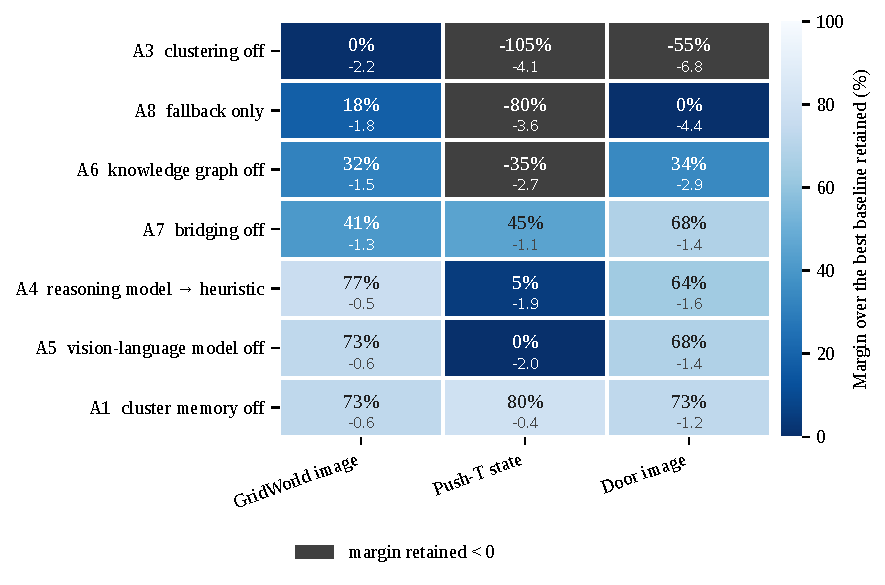
\includegraphics[width=\columnwidth]{figures/knockout_summary.pdf}
\caption{Cost of each knockout in points of final success rate against full DISEIL,
averaged over the three ablation settings. The partition knockout is the most damaging;
the remaining components cost gaps comparable to the seed standard error of the full
run.}
\label{fig:knockoutsummary}
\end{figure}

\begin{table*}[t]
\centering
\caption{Every knockout, on the three ablation settings, ordered by mean damage.
Values are the change in final success rate in points against full DISEIL. Mean margin
retained is the mean over the three settings of
$(\text{ablated} - \text{best baseline}) / (\text{full} - \text{best baseline})$, as a
percentage. A negative value means the ablated system finished, on average, beneath the
baseline it was built to beat. GW is GridWorld (image), PT is Push-T (state) and Dr is
Door (image).}
\label{tab:knockouts}
\begin{tabular}{llrrrrr}
\toprule
 & & \multicolumn{3}{c}{$\Delta$ success rate (points)} & & Mean margin \\
\cmidrule(lr){3-5}
Study & Component knocked out & GW & PT & Dr & Mean & retained (\%) \\
\midrule
A3 & the clustering step & $-2.2$ & $-4.1$ & $-6.8$ & $-4.37$ & $-53.2$ \\
A8 & the prescription, fallback rule promoted & $-1.8$ & $-3.6$ & $-4.4$ & $-3.27$ & $-20.6$ \\
A6 & the environmental constraints & $-1.5$ & $-2.7$ & $-2.9$ & $-2.37$ & $10.3$ \\
A4 & the prescription model & $-0.5$ & $-1.9$ & $-1.6$ & $-1.33$ & $48.6$ \\
A5 & the vision-language model & $-0.6$ & $-2.0$ & $-1.4$ & $-1.33$ & $47.0$ \\
A7 & bridging placement & $-1.3$ & $-1.1$ & $-1.4$ & $-1.27$ & $51.4$ \\
A1 & the cluster memory & $-0.6$ & $-0.4$ & $-1.2$ & $-0.73$ & $75.1$ \\
\bottomrule
\end{tabular}
\end{table*}

\begin{table}[t]
\centering
\caption{The allocation ladder in absolute terms: final held-out success rate (per
cent) on the three ablation settings. A2 replaces allocation with a uniform draw over
recorded failures, A8 promotes the deterministic fallback rule to the whole method,
and A3 keeps the loss signal and removes the mode structure. GW is GridWorld (image),
PT is Push-T (state) and Dr is Door (image).}
\label{tab:ladder}
\begin{tabular}{llrrr}
\toprule
 & Arm & GW & PT & Dr \\
\midrule
A2 & uniform-random allocation & 89.1 & 82.3 & 80.0 \\
A8 & fallback rule only & 89.5 & 92.5 & 84.2 \\
A3 & greedy worst-loss & 89.1 & 92.0 & 81.8 \\
 & full DISEIL & \textbf{91.3} & \textbf{96.1} & \textbf{88.6} \\
\bottomrule
\end{tabular}
\end{table}

\begin{figure}[t]
\centering
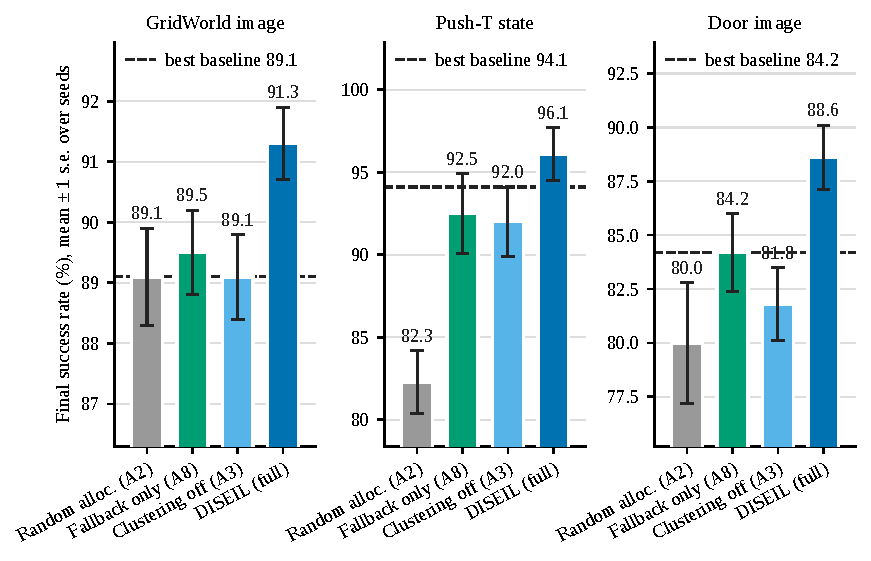
\includegraphics[width=\columnwidth]{figures/allocation_ladder.pdf}
\caption{The allocation ladder on the three ablation settings. Bars are the mean final
success rate over seeds with one standard error, for uniform-random allocation over
recorded failures (A2), the deterministic nearest-untried fallback rule promoted to the
whole method (A8), clustering removed in favour of greedy worst-loss selection (A3),
and full DISEIL. The dashed line is the strongest baseline in that setting. Budget
$B = 20$, one demonstration per round.}
\label{fig:ladder}
\end{figure}

\paragraph{A2, uniform-random allocation.} The first rung corrects one uniformly chosen
recorded failure each round, with no descriptor, no partition, no memory and no
prescription model. On GridWorld this arm is the Stagger control of the main results
table; on the robot settings it is a separate run. It reaches 89.1, 82.3 and 80.0
against DISEIL's 91.3, 96.1 and 88.6. On the two robot settings it lands well below the
strongest gated baseline. On GridWorld (image) it finishes level with the gated
baselines and marginally above the best of them, and still below DISEIL.

Sampling failures uniformly reproduces the frequency of failure modes in the current
policy's failure set, so the dominant mode is corrected in proportion to how often it
occurs and a rare, persistent mode is almost never touched inside twenty rounds. The
premise of the whole framework is that the value of a demonstration is not proportional
to the frequency of the corresponding failure, and A2 measures that premise directly.
It also settles the obvious objection, that the advantage is nothing more than failure
replay. On the robot settings random replay is worse than an uncertainty gate, and an
uncertainty gate is worse than allocation; on the small GridWorld task the gates and
random replay finish level, and allocation still leads.

\paragraph{A8, the deterministic fallback rule.} When the prescription model cannot
produce a feasible prescription after five attempts, DISEIL falls back on the nearest
untried recorded failure in descriptor space. A8 promotes that rule to the entire
method. It reaches 89.5, 92.5 and 84.2, costs 1.8, 3.6 and 4.4 points, and retains
18.2, $-80.0$ and 0.0 per cent of the margin. It beats the strongest baseline on
GridWorld (image) only; on Push-T (state) it falls below it, and on Door (image) it
lands exactly on it.

Nearest-untried is a spatial heuristic that implicitly spreads the budget, since a
failure adjacent to one already corrected is less likely to be chosen than a distant
one, and that is a crude version of the coverage pressure the partition and the memory
supply deliberately. It captures a fraction of the margin at best, and it turns
negative on Push-T (state), the setting whose strongest baseline is itself the
strongest in the main results table. It cannot do better, because nearest-untried has
no notion of a failure mode: it will select a chain of adjacent failures that all
belong to the same mode, and it has no mechanism for concluding that a mode has been
addressed. A8 is the floor against which every claim about the language and
vision-language components is calibrated, alongside the baselines rather than in place
of them.

\paragraph{A3, the clustering step, and the dissociation.} The third rung removes the
clustering step and targets, each round, the single failure with the highest peak
per-step loss. The loss signal is kept and the failure-mode structure is removed.
Success falls by 2.2, 4.1 and 6.8 points, a mean of 4.37, and the margin retained
collapses to 0.0, $-105.0$ and $-54.5$ per cent, a mean of $-53.2$. On Push-T (state)
and Door (image) the ablated system falls beneath its own best baseline, 92.0 against
94.1 and 81.8 against 84.2, and on GridWorld (image) it lands exactly on it. Removing
the clustering step erases the whole margin and on two of the three settings turns it
negative, the largest damage of any knockout in the programme.
Figure~\ref{fig:gainalloc} plots the arm against its baselines.

\begin{figure}[t]
\centering
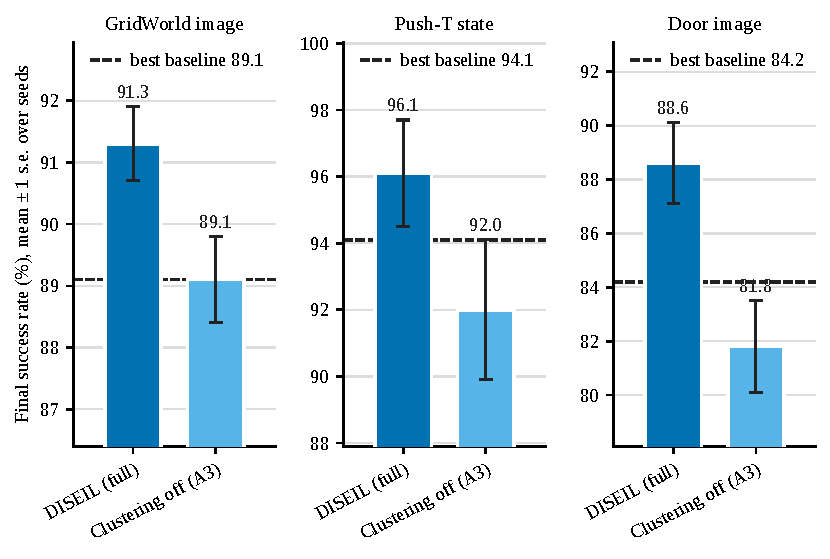
\includegraphics[width=\columnwidth]{figures/gain_without_allocation.pdf}
\caption{Success rate with clustering removed. Final success rate for full DISEIL and
for greedy worst-loss selection (A3) on the three ablation settings, with the strongest
baseline as a dashed line.}
\label{fig:gainalloc}
\end{figure}

What makes A3 the argument of the paper, and not one knockout among seven, is what
happens to the information gain while the success rate is falling by those amounts.
Per-demonstration information gain does not fall when clustering is removed. It rises
on two of the three settings, by 0.02 and 0.16, and falls on the third by 0.13, for a
mean change of $+0.02$. Greedy worst-loss selection is as good as DISEIL, or marginally
better, at collecting demonstrations on which the current policy has high pre-retrain
loss, which is unsurprising, since maximising that quantity is exactly what it does by
construction, whereas DISEIL sacrifices some of it to spread the budget across failure
modes. The two quantities move in opposite directions, and the dissociation is the
finding.

The mechanism is straightforward once stated. Peak loss is a property of one failure
trajectory. It is not a property of the \emph{set} of failures the policy is still
producing. Under greedy worst-loss, the highest-loss failure in round $r$ very likely
belongs to the same failure mode as the highest-loss failure in round $r-1$, because
the modes that generate the largest loss spikes are the ones the policy has learned
least about, and one demonstration does not close a mode. The budget is spent
repeatedly inside one region of the state space. Each demonstration in that stream is
genuinely informative in isolation, which is why the gain does not fall, and each is
largely redundant with the demonstration collected in the round before, which is why
the success rate does not move. Figure~\ref{fig:infogain} shows the per-setting
distribution of the quantity that the main paper's information-gain table summarises.

The main paper's table reproduces Diff-DAgger alone as the comparison column, because
Diff-DAgger's gate selects on the same per-step diffusion loss the metric is computed
from and is therefore the one baseline that could be expected to lead on it. The four
other query gates and the uniform-random control are not reproduced as columns, and
they add no argument the Diff-DAgger column does not already make: DISEIL's mean gain
is above every gate in all ten settings, GridWorld included, and above the control
wherever the control was run.

\begin{figure*}[t]
\centering
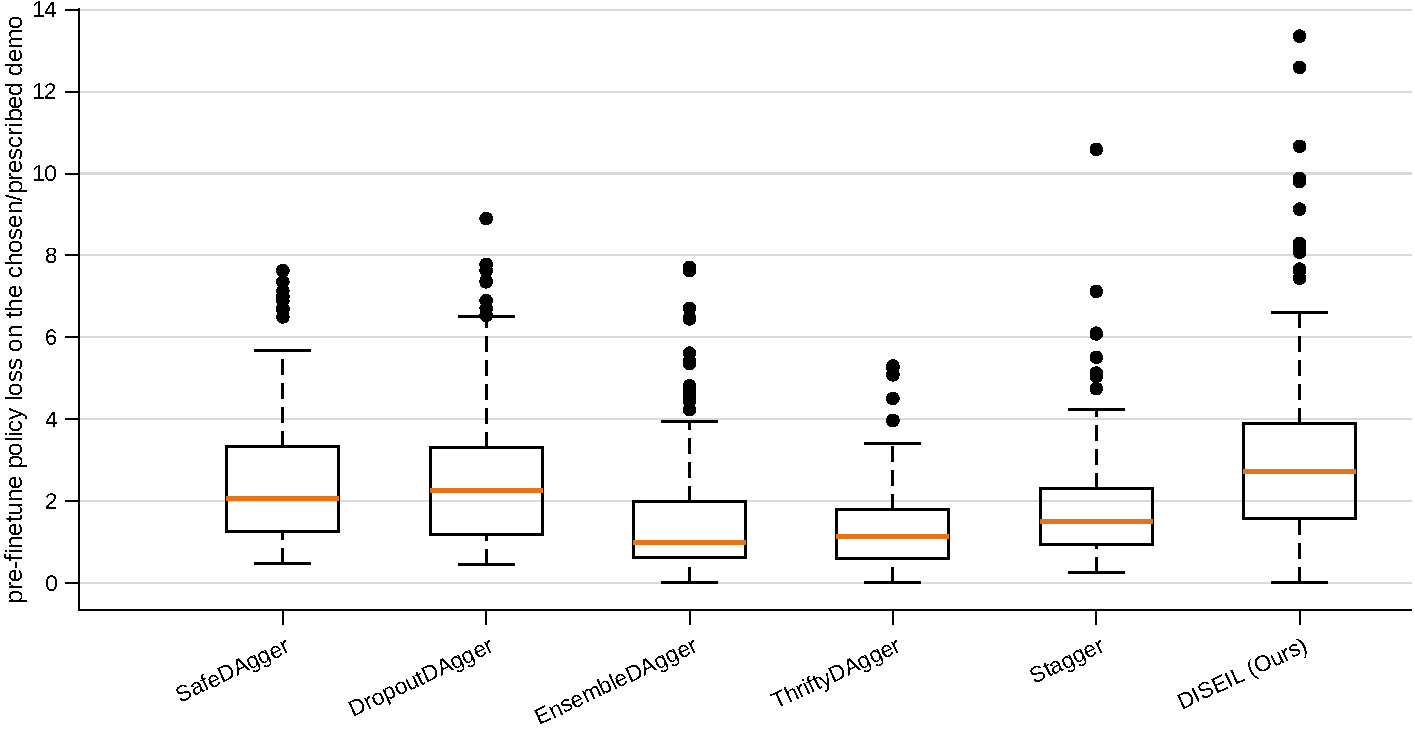
\includegraphics[width=\textwidth]{figures/info_gain.pdf}
\caption{Per-demonstration information gain, the policy's per-step loss on each newly
acquired demonstration measured before retraining on it. The distributional view of the
information-gain table in the main paper. Diff-DAgger is run on the robot tasks only.}
\label{fig:infogain}
\end{figure*}

A3 carries a limitation that is stated rather than deferred. It removes the descriptor
and the memory along with the clustering, because those components have nothing to
operate on once modes are gone, so it is a knockout of the allocation \emph{stack} and
not of the partition in isolation. The cleaner variant, which keeps the descriptor and
replaces agglomerative clustering \citep{ward1963hierarchical} with a random partition
of the failures into $k$ groups, would separate grouping by geometry from grouping at
all. It was not run, and it is future work rather than a claim.

\paragraph{A6, the constraints the prescription is checked against.} The prescription
model proposes a configuration; constraints are retrieved from the task's store, which
holds workspace bounds, reachability, object and spawn ranges and controller limits as
structured key-value knowledge; the proposal is checked against them; a violation is
returned to the model as feedback and a revised proposal is requested until a feasible
one is produced. A6 removes the store from both the vision-language and the reasoning
prompts, so the loop has nothing to verify against.

The cost is 1.5, 2.7 and 2.9 points, a mean of 2.37, and 31.8, $-35.0$ and 34.1 per
cent of the margin is retained, a mean of 10.3. A6 is the third most damaging knockout
and it costs nearly twice what the prescription model itself is worth. The fallback
rate rises to 27.1, 27.0 and 34.8 per cent of rounds, which means roughly five to seven
of the twenty rounds are spent on a fallback correction rather than a prescribed one, a
direct loss of a quarter to a third of the budget. Figure~\ref{fig:grounding} shows
both halves of the measurement.

\begin{figure}[t]
\centering
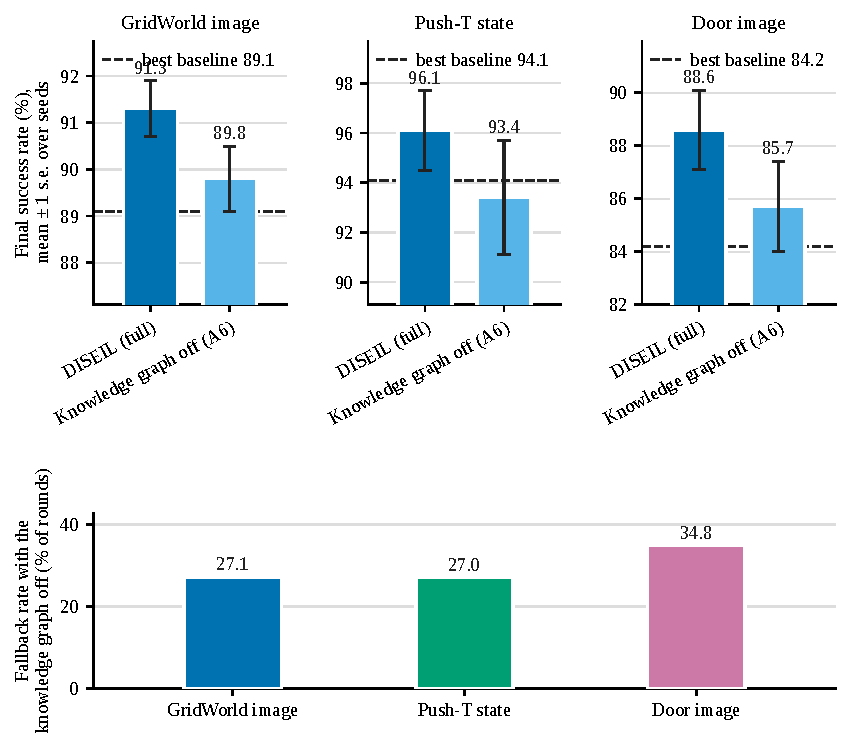
\includegraphics[width=\columnwidth]{figures/grounding_and_feasibility.pdf}
\caption{Grounding and feasibility. Top row: final success rate for full DISEIL and
with the environmental constraints removed from the prompts (A6), against the strongest
baseline. Bars are means over seeds with one standard error, including the A6 bar.
Bottom row: the share of rounds that fall back to the deterministic rule when the
constraints are removed.}
\label{fig:grounding}
\end{figure}

The relation between the fallback rate and the damage is loose, and A8 is what explains
it: a fallback round acquires the nearest untried failure, so a lost
round still costs the difference between a prescribed correction and a fallback correction and
not the whole round, which is why A6 costs two and a half points and not six. What the
store buys follows from the same mechanism. It stops the prescription model from
producing requests the environment cannot instantiate, and it does not make the model a
better reasoner. Two limitations bound the claim. The per-task store is authored by
hand and the study does not decompose it, so it cannot be said whether the workspace
bounds alone would recover most of the damage or whether the failure taxonomy and the
per-mode rules matter as well. And A6 knocks out only the first of the two screens; the
solvability screen is not ablated anywhere.

\paragraph{A4 and A5, the two model roles.} The \emph{prescription model} is the
text-only model of the main paper, and it fills two roles. In the first it assigns a
root cause and a trajectory phase to each failure, once per failure, from the taxonomy
stored in the task's constraint store. In the second it turns the selected mode and its
context set into the round's demonstration request, once per round. A4
replaces the second of those with the deterministic rule ``always target the dominant
cluster representative'', operating on the same geometric clusters, so that the
comparison isolates the prescription decision and not the partition; the root-cause
labelling role is retained in A4 and still runs. A5 removes the vision-language model,
leaving the prescription model with the geometric descriptor and the root-cause taxonomy.
The two roles are removed together nowhere in the programme, and the phrase
\emph{reasoning stack} names both roles of the prescription model plus the
vision-language call taken
together. Figure~\ref{fig:reasoning} plots both arms.

\begin{figure}[t]
\centering
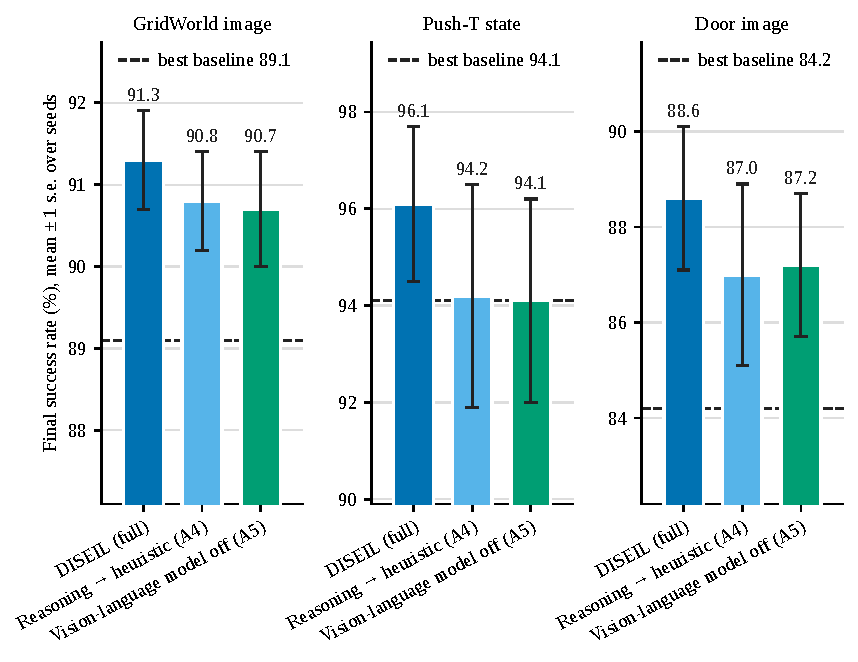
\includegraphics[width=\columnwidth]{figures/reasoning_and_vision_small.pdf}
\caption{The prescription model and the vision-language model. Final success rate for
full DISEIL, for the prescription model replaced by the dominant-representative
heuristic (A4), and for the vision-language model removed (A5), with one standard error
over seeds and the strongest baseline as a dashed line.}
\label{fig:reasoning}
\end{figure}

A4 costs 0.5, 1.9 and 1.6 points and A5 costs 0.6, 2.0 and 1.4, so both average 1.33
points and both retain roughly half the margin, 48.6 per cent for A4 and 47.0 for A5.
Every individual gap in both studies is comparable to the seed standard error of the
corresponding full run, and the two are close enough in magnitude that the study cannot
rank them. Both are largest on Push-T (state) and smallest on GridWorld (image).

The explanation is structural. Clustering is geometric in every run, state and image
alike, and it consumes no output from any foundation model. By the time either model is
called, the decision that matters, which region of the failure distribution receives
this round's demonstration, has already been made by the descriptor and the memory. The
prescription model chooses the form of the correction inside a region that was selected
without it. A component acting downstream of the decisive step cannot produce a large
effect, and the measurement agrees. Read the other way, the same fact is a practical
result: a deployment that cannot afford the reasoning stack can delete it, keep the
geometric clustering, the memory and the deterministic heuristic, and still beat every
baseline on every setting.

Both knockouts carry a limitation that cuts against the framework's interest. The A4
heuristic is a strong one. ``Always target the dominant cluster representative'' is itself
an allocation rule, and it inherits the memory's rotation, because the dominant cluster
changes as the memory penalises recently corrected regions. A weaker heuristic would
have produced a larger gap. The heuristic also cannot bridge, so A4 and A7 are not
independent, and the study cannot separate what the prescription model buys as a
reasoner from what it buys as the only component that can place a demonstration between
two failures. A5, for its part, does not test whether a better visual model would help
more. Its largest gap is on Push-T (state), a state-modality setting and therefore
counterintuitive, and the reading the architecture supports is that the frames are not
there to compensate for a missing state vector. They are there to let the model see why
the block ended where it did, and Push-T is the task on which one terminal geometry can
be reached by several distinct failure processes, such as pushing on the wrong face,
losing contact, or over-rotating. On Door, where the geometry of a failure largely
determines its cause, the visual channel adds less.

\paragraph{A7, bridging placement.} Bridging is the only part of the prescription that
changes the environment configuration rather than selecting an episode, and it is the
mechanism by which a prescription can be made easier than the failure it addresses.
Disabling it costs 1.3, 1.1 and 1.4 points, a mean of 1.27, and retains 40.9, 45.0 and
68.2 per cent of the margin. That is proportionate to how often the arm is used: the
bridged share of accepted prescriptions, measured as diagnostic A16 and shown in
Figure~\ref{fig:bridging}, is 24, 28 and 21 per cent. A component used in a quarter of
rounds cannot produce a large aggregate effect unless the rounds in which it is used
are the decisive ones, and the three settings do not order the damage the way they
order the share: the largest damage is on the setting with the middle share. What
matters is which rounds bridge and not how many, and the coherent reading is that
bridging pays when the target cluster lies far outside anything the current policy
solves, so that a targeted demonstration would be a large distributional jump and a
bridged one is a step the policy can absorb. That reading is not itself tested here.

\begin{figure}[t]
\centering
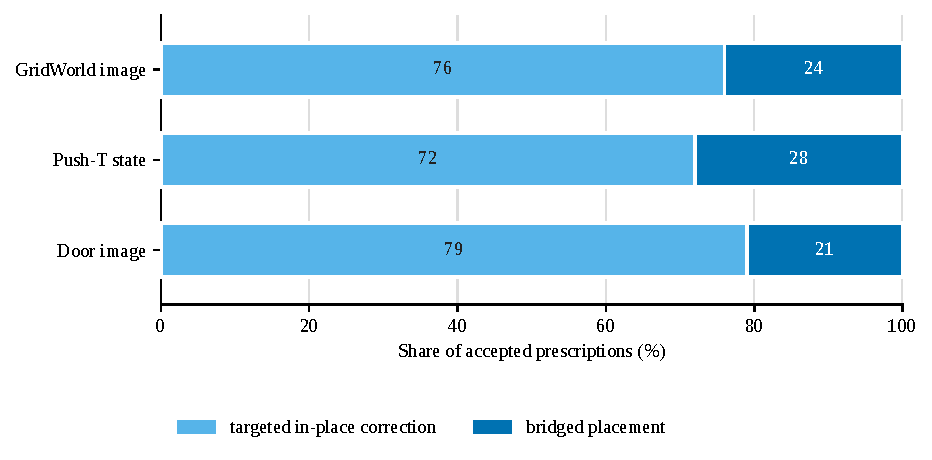
\includegraphics[width=\columnwidth]{figures/bridging.pdf}
\caption{Targeted and bridged prescriptions (study A16). Share of accepted
prescriptions on each of the three ablation settings that are a targeted in-place
correction and that are a bridged placement.}
\label{fig:bridging}
\end{figure}

\paragraph{A1, the cluster memory.} Switching the memory off, $\lambda = 0$, costs 0.6,
0.4 and 1.2 points, a mean of 0.73, and retains 72.7, 80.0 and 72.7 per cent of the
margin, a mean of 75.1. It is the smallest effect of the seven knockouts and every
individual gap is no larger than the seed standard error of the corresponding full run.
The memory suppresses a cluster that has just received a demonstration, so the
following round is pushed onto a different one, and A1 prices that suppression once the
partition is already in place. The price is task-dependent: 0.4 points on Push-T
(state) and 1.2 on Door (image), a factor of three across two of the three settings, so
no single number describes what the memory is worth and the study does not supply one.
The framework carries the memory as a configurable component of the loop, switched on
per task, and not as a headline contribution. This study is the evidence for that
description. What the framework has to defend is the partition the memory operates
over, and A3 is where it is defended.

The kernel is also inert in most rounds. The candidate set of near-dominant modes is a
singleton in 56 to 84 per cent of rounds on the settings with enough telemetry, and the
dominant mode is then returned regardless of the penalty. The bandwidth is a single
global constant while the tasks do not share a spatial scale. The memory is switched on
in every run reported in the main paper and it is not drawn in the architecture figure.

\paragraph{The ordering.} Ranked by mean damage, the seven knockouts are: clustering
($-4.37$ points, $-53.2$ per cent of the margin retained), the fallback rule promoted to
the whole method ($-3.27$, $-20.6$), the constraint store ($-2.37$, $10.3$), the
prescription model and the vision-language model ($-1.33$ each, $48.6$ and $47.0$),
bridging placement ($-1.27$, $51.4$) and the cluster memory ($-0.73$, $75.1$). The
ordering shaped the rest of the programme in two ways. The clustering step, which the
framework treats as an implementation detail of a generic partition, is the component
that carries the result. The cluster memory, which an earlier draft of the method
advanced as one of its two contributions, is the least damaging of the seven and is
reported as a configurable, task-dependent feature on that evidence.

\section{G. Design Choices, A9 to A13}

Given that allocation is the mechanism, the next family of studies asks whether
\emph{this} descriptor, \emph{this} cluster count, \emph{this} context set and
\emph{this} budget are the right way to allocate. These studies were added after the
knockouts, because until the knockouts had run there was no reason to interrogate the
partition in such detail.

\paragraph{A10, the width of the descriptor.} The descriptor is designed, not learned,
which invites the suspicion that the feature set was fitted to the reported result. A10
answers by scoring the descriptor on what it is for, the separation of failure modes,
using a criterion with no relationship to success rate: the mean silhouette of the
resulting clusters \citep{rousseeuw1987silhouette}. Features are removed from and added
to the descriptor and the silhouette is measured over every clustering round. If the
feature set had been over-specified, the curve would be flat and the choice of six
dimensions arbitrary.

\begin{table}[t]
\centering
\caption{Mean silhouette of the failure clusters against the width of the geometric
descriptor (study A10), averaged over the three ablation settings. Six dimensions is
the highest-scoring variant in each of the three settings individually. Silhouette
scores geometric separation only and is independent of the success rate.}
\label{tab:descdim}
\begin{tabular}{lr}
\toprule
Descriptor dimensions & Mean silhouette \\
\midrule
2 & 0.373 \\
4 & 0.507 \\
5 & 0.557 \\
6 (the framework's setting) & \textbf{0.593} \\
8 & 0.550 \\
10 & 0.490 \\
12 & 0.423 \\
\bottomrule
\end{tabular}
\end{table}

\begin{figure}[t]
\centering
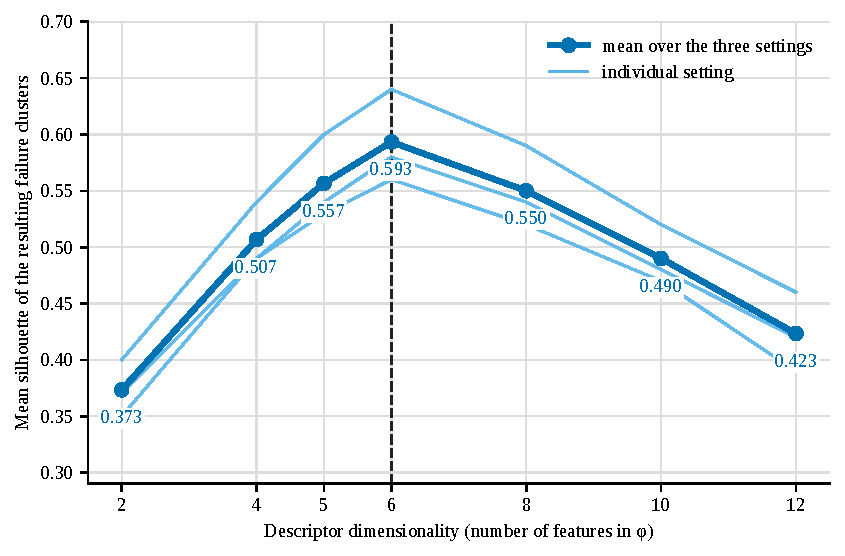
\includegraphics[width=\columnwidth]{figures/descriptor_dimensionality.pdf}
\caption{Mean silhouette of the failure clusters against the dimensionality of the
geometric descriptor. One line per ablation setting and the mean over the three. The
dashed vertical line marks the six-dimensional descriptor the framework uses.}
\label{fig:descdim}
\end{figure}

The curve is a clean inverted U with a single interior maximum, and the six-dimensional
descriptor is the highest-scoring variant in each of the three settings.
Table~\ref{tab:descdim} gives the mean and Figure~\ref{fig:descdim} the per-setting
curves. Below six dimensions the descriptor discards information that distinguishes
modes, and the largest single step in the whole sweep, $+0.133$ in mean silhouette, is
the step from two dimensions to four, which adds orientation. Position alone cannot
separate a Push-T failure in which the block is in the right place at the wrong angle
from one in which it is in the right place at the right angle and the pusher lost
contact, so those failures collapse into one cluster and the cluster's silhouette is
poor. Adding task progress, worth $+0.050$, and contact distance, worth $+0.037$, each
buy less, which is consistent with orientation being the dominant discriminator on
these tasks.

Above six dimensions the fall is not an information loss, since every added feature
carries some signal. It is geometric. As dimensionality rises, the ratio of the nearest
to the farthest pairwise distance approaches one, all failures come to look
equidistant, the agglomerative merge order becomes arbitrary, and the silhouette falls
although nothing was removed. End-effector velocity adds two dimensions of mostly noise
to a distance computation over a few dozen points, and by twelve dimensions the
joint-angle summary has added six more. The number of failures being clustered is
small, forty-two in round 1 and two by round 20 on the instrumented setting, and
distance concentration bites hardest at small sample sizes. The descriptor is small
because the failure sets are small, and the two facts are linked by the geometry of the
distance computation and not by a design preference.

A10 also settles a point of record. Clustering is geometric for every run, state
modality and image modality alike, and the descriptor is the same six-dimensional
vector in both. The limitation is the one silhouette cannot address: it scores
geometric separation and not semantic correctness, and a descriptor could produce
well-separated clusters that correspond to no distinct root causes at all. The purity
diagnostic of Section H is the measurement that bears on that hole and it does not close
it. A10 also shows only that this family of descriptors peaks at six dimensions. It says
nothing about whether a learned descriptor would do better.

\paragraph{A9 and A13, the context set.} The context set given to the prescription model
contains three cited failure episodes chosen by three rules: the forced representative
of the target cluster, the worst-peak-loss seed, and a farthest-point-sampling fill for
diversity \citep{eldar1997fps}. Written out, the set $S$ referred to in the main paper's
Prioritise stage is built from the target mode $C_{\mathrm{tgt}}$ as
%
\begin{equation}
\label{eq:context}
\begin{aligned}
S_0 &= \big\{\mathrm{rep}(C_{\mathrm{tgt}})\big\} \cup \Big\{\arg\max_{i \in
C_{\mathrm{tgt}}} \mathrm{peak}_i\Big\}, \quad S \leftarrow S_0, \\
S &\leftarrow S \cup \Big\{ \arg\max_{i \in C_{\mathrm{tgt}} \setminus S} \
\min_{j \in S} \ \big\| \tilde{X}_i - \tilde{X}_j \big\|_2 \Big\} \\
&\qquad \text{ until } |S| = \min\big(\kappa,\, |C_{\mathrm{tgt}}|\big),
\end{aligned}
\end{equation}
%
with $\kappa = 3$ in every reported run and $\tilde{X}$ the standardised descriptors.
A9 removes each rule in turn and adds a floor control of
three episodes drawn at random from the cluster, with the target cluster fixed by the
memory in every arm so that only the composition of the set varies. All figures in this
paragraph are means over the three ablation settings against a full-system reference of
92.0, and they are collected in Table~\ref{tab:context}.

\begin{table}[t]
\centering
\caption{The composition and the size of the context set (studies A9 and A13), as the
mean cost in success-rate points over the three ablation settings against a
full-system reference of 92.0. The single-citation arm was not run because bridging
requires at least two cited failures to define a placement, so it is confounded by
construction and is not a null result.}
\label{tab:context}
\begin{tabular}{lr}
\toprule
Arm & Cost (pts) \\
\midrule
\multicolumn{2}{l}{\emph{A9, composition; three citations}} \\
Drop the forced representative & $-3.2$ \\
Drop the diversity fill & $-3.2$ \\
Drop the worst-loss seed & $-3.27$ \\
Three episodes drawn at random & $-3.6$ \\
\midrule
\multicolumn{2}{l}{\emph{A13, number of citations}} \\
Top three by plain peak-loss rank & $-2.13$ \\
Two citations & $-1.93$ \\
Five citations & no gain \\
One citation & not run \\
\bottomrule
\end{tabular}
\end{table}

The three single-rule removals cost almost the same, so on this run the study cannot
rank the three rules against one another. Each still hurts, and each for a reason the
others do not cover. The forced representative guarantees the prescription model sees an
example of the mode it has been instructed to fix, without which the cited episodes can
all come from the cluster's periphery. The diversity fill keeps a context set of three
episodes from all crowding near the loss peak, where it would describe the mode narrowly
and draw a narrow correction. The worst-loss seed sharpens the description of the mode.
Random selection of three episodes costs 3.6 points, more than any single-rule removal,
so the three rules together beat an unstructured draw and are complementary rather than
redundant.

The magnitudes discipline the claim. The whole spread from the full context set to
random selection is 3.6 points, larger than the constraint store and still less than the
clustering. A13 sharpens the point by varying the \emph{number} of cited episodes
jointly with the selection rule, and it contains the one comparison that could have
deleted a component of the method: citing the top three episodes by plain peak-loss
rank, against the three-rule construction, at the same number of citations. The gap is
2.13 points. It is a real gap in the paired sense, since the full construction wins on
each of the three settings, so the farthest-point construction earns its place rather
than barely surviving. Citing only two episodes costs 1.93 points, so fewer citations
are worse; citing five gives no measurable gain over three; and citing every failure in
the target cluster only raises the prompt length without adding discriminative detail,
since the early rounds carry about forty failures and a context set of that size buries
the target mode in detail the model cannot weigh. The cap at three is therefore
justified from both sides. The single-citation arm was not run, and the reason is that
it is confounded by construction: bridging requires at least two cited failures in order
to define a placement between a failing region and a solved one. It is not a null result
and must not be reported as one.

\paragraph{A12, the cluster count.} The cluster count is chosen per round by maximum
mean silhouette, which is standard practice, is used as such, and is not claimed as a
contribution \citep{rousseeuw1987silhouette, pedregosa2011sklearn}. A12 replaces the
adaptive choice with a fixed $k$. Silhouette selection wins on each of the three
settings, and it beats the best fixed alternative, averaged over the three, by 4.1
points: a fixed $k = 2$ costs 4.1 points against the adaptive rule, $k = 3$ costs 4.6,
$k = 4$ costs 7.4 and $k = 5$ costs 6.7. The effect is well outside the seed standard
error of the three settings, which runs from 0.6 to 1.6 points, so the adaptive rule is
defended by the size of its effect and not only by the consistency of its sign.

No single fixed $k$ is best across the three settings either: the best fixed value is
$k = 3$ on GridWorld (image), $k = 2$ on Push-T (state) and $k = 5$ on Door (image),
which is the point. Too few clusters merges distinct failure modes, so the memory
penalises a merged cluster and suppresses correction of a mode that was never addressed.
Too many splits one mode across several clusters, so the memory cannot recognise that
the mode has been corrected and rotation is diluted across fragments of the same region.
The right number varies by setting and by round, and only the adaptive rule tracks it.
Figure~\ref{fig:context} plots A9, A12 and A13 together.

\begin{figure}[t]
\centering
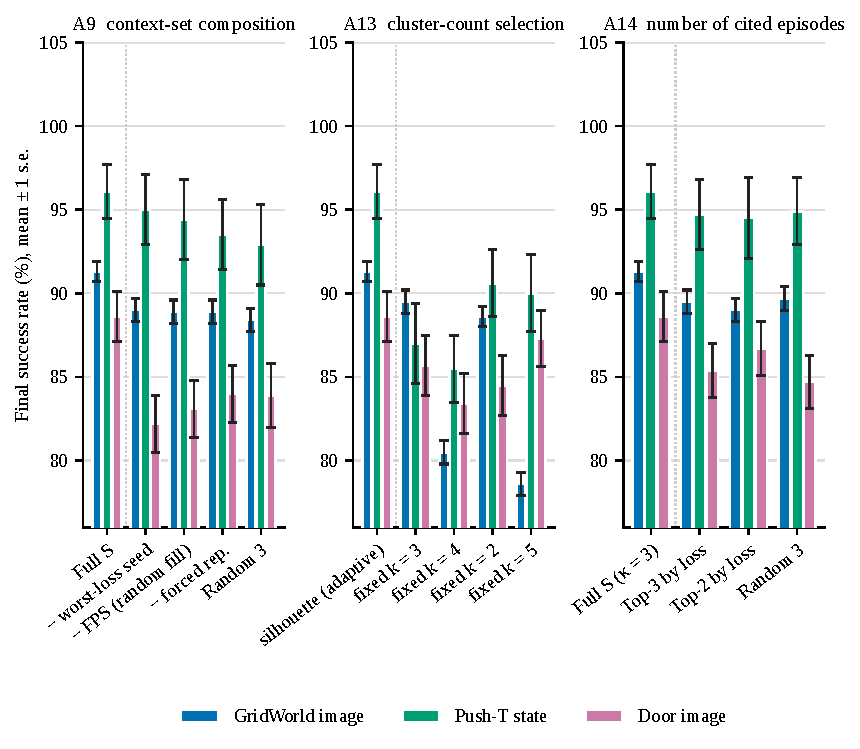
\includegraphics[width=\columnwidth]{figures/context_and_selection.pdf}
\caption{Three ablations of the machinery inside individual steps, with arms ordered by
effect. Left: the composition of the context set (A9). Middle: silhouette-based
selection of the cluster count against fixed alternatives (A12). Right: the number of
cited episodes and the selection rule (A13). Bars are means over seeds with one
standard error, on the three ablation settings.}
\label{fig:context}
\end{figure}

\paragraph{A11, the budget.} The framework is claimed to operate under any fixed budget,
with $B = 20$ as the validated instance, and A11 is the experiment that supports or
refutes the claim. The margin is far larger at the smallest budget than at the two
larger ones: it averages $+9.07$ points at $B = 10$, $+2.87$ at $B = 20$ and $+2.83$ at
$B = 40$, with per-setting values of $+5.7$, $+9.0$ and $+12.5$ at the smallest budget
and $+1.5$, $+3.2$ and $+3.8$ at the largest. The decline is clean on GridWorld (image)
and Door (image); on Push-T (state) the margin is $+9.0$ at $B = 10$ and then sits near
two to three points at the two larger budgets, so the trend is not strictly monotonic
there.

The margin shrinks because the baseline catches up and not because DISEIL degrades, and
Figure~\ref{fig:budget} is the evidence. DISEIL's own success rate rises with the budget
on every one of the three settings, from 86.8 to 94.0 on GridWorld (image), from 87.9 to
97.7 on Push-T (state) and from 82.3 to 99.5 on Door (image), while the strongest
baseline rises faster from a lower start. Allocation buys the \emph{rate} at which the
failure distribution is covered and not the asymptote, which is why a large budget
closes the gap: with enough draws, even a poorly allocated stream eventually covers the
failure distribution, because coverage is a coupon-collector problem and the collector
wins if it draws long enough.

\begin{figure}[t]
\centering
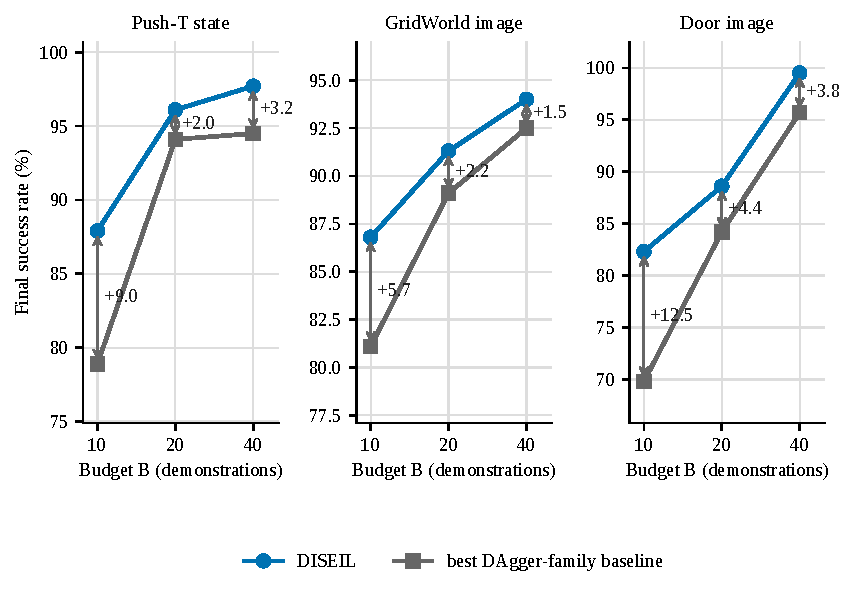
\includegraphics[width=\columnwidth]{figures/budget_sweep.pdf}
\caption{Final success rate against the budget $B$ (study A11). DISEIL against the
strongest baseline at $B = 10$, 20 and 40, on the three ablation settings, with the
margin printed between the two series.}
\label{fig:budget}
\end{figure}

One claim the sweep was expected to support does not hold, and it is retracted here. The
study was designed around the headline that DISEIL at $B = 10$ matches the strongest
baseline at $B = 20$, which would be the same policy for half the expert labour. It does
not. On the three ablation settings, DISEIL at $B = 10$ reaches 86.8 against the
baseline's 89.1 at $B = 20$ on GridWorld (image), 87.9 against 94.1 on Push-T (state)
and 82.3 against 84.2 on Door (image), so it falls short on every one. The halved-labour
claim is false and appears nowhere in either document. What survives is the claim the
data do support, which is the one that matters: the advantage of allocation grows as the
budget shrinks, and the method stops paying when demonstrations stop being scarce.

\section{H. Diagnostics, A14 to A17}

The last family of studies removes nothing. It asks whether the clusters the framework
discovers mean what the method says they mean, and whether the machinery that discovers
them stays active for as long as the budget runs. Both answers bound the claims above
rather than adding to them.

\paragraph{A14, and the limit of a geometric descriptor.} A10 shows that the descriptor
produces well-separated clusters. A well-separated cluster need not correspond to a
single root cause, and A14 is the check that stops the failure-mode claim from being a
statement about geometry alone. Purity runs from 0.84 to 0.91 across the three settings
and the number of distinct root causes per cluster runs from 1.35 to 1.86.
Table~\ref{tab:purity} gives the grid.

\begin{table}[t]
\centering
\caption{Root-cause label purity per geometric cluster (study A14). Mean cluster purity
is the fraction of a geometric cluster's failures that share the dominant root cause
assigned by the prescription model. Mean root causes per cluster counts the distinct root
causes present in a cluster. Purity is scored against the prescription model's own labels,
so it records agreement between two components of the same system and not agreement
with ground truth.}
\label{tab:purity}
\begin{tabular}{lrrr}
\toprule
Setting & Purity & Causes & Silhouette \\
\midrule
GridWorld 5x5 (image) & 0.89 & 1.62 & 0.58 \\
Push-T (state) & 0.91 & 1.35 & 0.64 \\
Door (image) & 0.84 & 1.86 & 0.56 \\
\bottomrule
\end{tabular}
\end{table}

The ordering is the informative part and it is the same ordering on both columns.
Push-T (state) has the best silhouette, 0.64, and the highest purity, 0.91. Door (image)
has the lowest silhouette, 0.56, the lowest purity, 0.84, and the most root causes per
cluster, 1.86. Geometric separation and semantic purity rise and fall together on these
three settings, so A10 and A14 are not independent audits of the descriptor: a
descriptor that separates well geometrically also tends to produce clusters that are
semantically clean, and neither measurement checks the other. What A14 establishes is
the qualification and not an independent guarantee. The descriptor separates failures by
where and how they occur, and it recovers root cause only to the extent that
configuration determines cause. Where several causes share one end-effector position, as
they do wherever a cluster carries close to two distinct root causes, geometry cannot
tell them apart.

The circularity in the measurement is admitted. Purity is scored against the reasoning
model's own root-cause labels, so it records agreement between two components of the
same system. There is no human-labelled root-cause set, and there should be, because
purity and silhouette covary and a human-labelled set is the only measurement that would
audit either of them from outside.

\paragraph{A15, the distribution of the cluster count.} A15 shows that the adaptivity is
not a disguised constant. Pooled over the 308 clustered rounds of the three ablation
settings, $k = 3$ is the most frequently selected count at 26.3 per cent, with $k = 4$
at 23.4, $k = 5$ at 21.4, $k = 2$ at 14.9 and $k = 6$ at 14.0. No value from two to six
falls below 14 per cent. The claim the framework may make is that the number of
discovered failure modes varies by round and is most often three or four, and not that
there are three failure modes.

A15 also carries a seam. Twenty-one per cent of GridWorld (image) rounds, 15 per cent of
Push-T (state) rounds and 20 per cent of Door (image) rounds never cluster at all,
because fewer than four failures remain, and in those rounds each failure becomes its
own cluster and the budget is allocated by the fallback rule. Figure~\ref{fig:kdist}
shows the distribution with those rounds marked.

\begin{figure}[t]
\centering
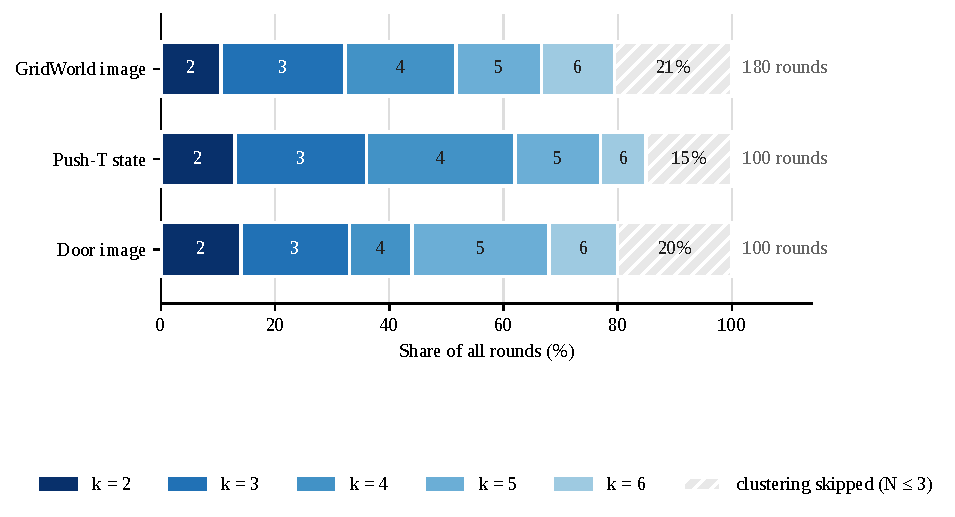
\includegraphics[width=\columnwidth]{figures/cluster_count_distribution.pdf}
\caption{Cluster count selected per round (study A15). Share of all rounds selecting
each cluster count $k$, with the rounds that skip clustering entirely, because fewer
than four failures remain, shown hatched.}
\label{fig:kdist}
\end{figure}

\paragraph{A16, the bridged share, and a discrepancy of record.} The share of accepted
prescriptions that are bridged is 24 per cent on GridWorld (image), 28 on Push-T (state)
and 21 on Door (image), plotted in Figure~\ref{fig:bridging} alongside study A7.

One discrepancy in the record is stated rather than smoothed over. The method's
precondition for bridging is pose randomisation, from which it follows that bridging
should be inapplicable on GridWorld, which is a discrete grid. The prescription logs
disagree: 24 per cent of accepted prescriptions on GridWorld (image) are marked bridged,
and A7 records a measurable effect there. Either the implemented mechanism is broader
than the method text claims, or the runs did something the method text did not intend.
The data are the source of truth, so bridging is reported as active on that setting, and
the resolution of the discrepancy, by inspection of the prescription logs, is an
outstanding item listed in Section N.

\paragraph{A17, failures per round.} Failures per round fall from forty-two to two over
the budget, halving by round 8 and falling by an order of magnitude by round 17. The
decline is the system working as intended, and it also bounds the system's own
mechanism. Clustering forty failures into three or four failure modes is a meaningful
operation. Clustering five failures into three is barely one. On the instrumented
setting the descriptor, the clustering and the memory do their work through round 17,
and the last three rounds run the fallback rule on a handful of remaining failures. A15
confirms the pattern on the three ablation settings, where 15 to 21 per cent of all
rounds skip clustering altogether. Figure~\ref{fig:failures} plots the curve.

\begin{figure}[t]
\centering
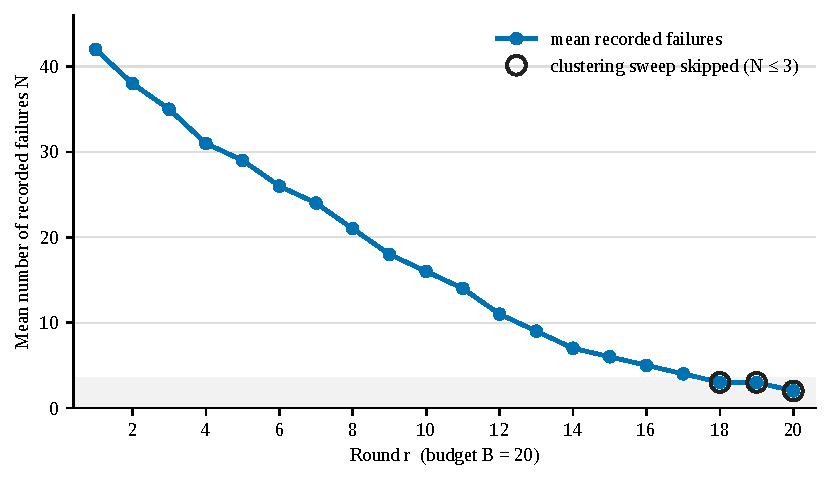
\includegraphics[width=\columnwidth]{figures/failures_over_budget.pdf}
\caption{Mean number of recorded failures per round over the budget (study A17). The
setting is Push-T (image), averaged over five seeds. Below four remaining failures the
clustering sweep is skipped and each failure becomes its own cluster; the shaded band
marks that region.}
\label{fig:failures}
\end{figure}

This diagnostic is instrumented on one setting, Push-T (image), the only setting for
which the failure count was logged per round. It is a diagnostic of the loop rather than
an arm of an ablation, and the instrumentation should be extended to the three ablation
settings before the front-loading behaviour is claimed as general, because the shape may
differ where the initial success rate is higher. That is an outstanding item.

Read alongside the budget sweep, where the margin more than triples as the budget is
halved, A17 says that DISEIL front-loads the value of a small budget, and the two facts
are consistent: the budget's marginal value is highest early and the machinery is most
active early. It also names an extension that is not tested here and is not claimed,
which is to stop the reasoning stack once the failure count drops below the clustering
threshold and spend the remaining rounds on the fallback, saving most of the per-round
reasoning cost at no measured loss.

\section{I. Computational Cost, A18}

The per-round cost of the reasoning pipeline is a limitation of this framework and it is
the first quantity a reader will ask for once the success rates are accepted. Study A18
measures it directly, so that the limitation is stated with a number attached.

\paragraph{The measurement.} Each of five settings runs a matched pair of runs, DISEIL
against SafeDAgger, on the same task, the same observation modality and the same
hardware, and the wall-clock and token cost of every round is read out of each run's own
telemetry. SafeDAgger is the baseline arm throughout. Two protocols are reported and
they must not be mixed. Protocol P1 reports the first round of each run. It is the only
protocol available in all five settings, and the first round holds the weakest policy
and therefore the most failures and the most model calls, so P1 is an upper bound on
steady-state cost rather than an average of it. Protocol P5 reports the mean and the
sample standard deviation over the language-model-active rounds of the runs that carried
a longer budget, matched arm for arm against the baseline's same-indexed rounds. The
spread quoted under P5 is the round-to-round spread inside a run. A P1 row and a P5 row
measure different objects and no reader should read one against the other.

\begin{table*}[t]
\centering
\caption{Per-round wall-clock and token cost, DISEIL against SafeDAgger (study A18).
\emph{Shared} is the part of the round that both arms pay: a from-scratch policy retrain
and a held-out evaluation. \emph{Add-on} is every DISEIL-specific stage of the round,
which is the failure-screening rollout together with clustering, the vision-language
call, the reasoning call, the prescription and the feasibility check, less the
query-gate rollout the baseline runs in its place. \emph{Tokens} is the sum of the
vision-language and language-model tokens drawn in the round. Token counts are not
comparable across rows, because the settings were served by different backends and the
hidden reasoning tokens are read directly from the usage record on some and recovered
from the billed completion length on others.}
\label{tab:cost}
\begin{tabular}{llrrrrr}
\toprule
Protocol & Setting & Baseline (s) & DISEIL (s) & Shared (s) & Add-on (s) & Tokens \\
\midrule
P1 & Door (state) & 737.0 & 1{,}054.0 & 783.0 & $+270.0$ & 11{,}511 \\
P1 & Door (image) & 1{,}247.0 & 1{,}474.0 & 1{,}180.0 & $+293.0$ & 11{,}379 \\
P1 & Wipe (image) & 1{,}468.0 & 2{,}195.0 & 1{,}491.0 & $+700.0$ & 9{,}560 \\
P1 & Push-T (image) & 688.0 & 1{,}891.0 & 652.5 & $+1{,}232.1$ & 82{,}116 \\
P1 & GridWorld (image) & 54.6 & 118.0 & 51.1 & $+62.6$ & 9{,}735 \\
\midrule
P5 & Door (state) & 532.6 $\pm$ 145.5 & 782.6 $\pm$ 183.5 & 547.8 & $+232.8$ & 10{,}929 \\
P5 & Door (image) & 1{,}034.2 $\pm$ 150.2 & 1{,}168.8 $\pm$ 194.8 & 901.6 & $+266.2$ & 10{,}787 \\
P5 & Wipe (image) & 1{,}303.3 $\pm$ 144.1 & 1{,}991.0 $\pm$ 179.2 & 1{,}332.7 & $+655.7$ & 10{,}118 \\
\bottomrule
\end{tabular}
\end{table*}

\paragraph{What the measurement says.} A round's wall-clock is dominated by the
from-scratch policy retrain and the held-out evaluation, and both arms pay all of it.
Under P1 that shared cost is 783 to 1,491 seconds per round on the three RoboSuite
settings, against a reasoning add-on of 270 to 700 seconds, and under P5 it is 548 to
1,333 seconds against an add-on of 233 to 656. The ratio of a DISEIL round to a baseline
round inherits the large shared denominator and is diluted by it: across the two
protocols it runs from 1.13 to 2.75, and a ratio near one is not evidence that the
reasoning pipeline is cheap. It is evidence that the retrain is expensive. The quantity
that characterises the pipeline is the add-on, the seconds and the tokens the baseline
never spends, which is 63 seconds per round on GridWorld and 1,232 on Push-T, at 9,560
to 82,116 tokens per round. Both numbers belong in the record and neither on its own is
honest.

Push-T is the outlier and its reasoning is not the reason. Its shared cost is the second
smallest in the sweep and its baseline arm is unusually cheap, because SafeDAgger's loop
runs until the intervention budget is spent and therefore halts after its first
intervened episode, which is one episode and 6.3 seconds, while DISEIL screens a fixed
sixty. At a longer budget the baseline would roll out many episodes per retrain and the
ratio would fall. The token draw is the second reason: Push-T issues twenty
language-model calls against Door's seven. GridWorld sits at the other end in seconds
and not in tokens. Its whole round is 118 seconds, so 63 seconds of reasoning is more
than double a 55-second baseline round, and it still draws 9,735 tokens, of which the
constraint block is 54 per cent of the prompt budget, the largest share of any setting.
A cheap task in seconds is not a cheap task in tokens.

\paragraph{What this means for the framework.} The language and vision-language models
run only at demonstration-selection time. They are never in the control loop and they do
not run at execution, so their cost is paid once per round, and on the three RoboSuite
settings it is amortised over a retrain and an evaluation that together cost more than
the reasoning does. The resource being traded is model inference against expert
demonstration time, and on the settings measured here a round buys one demonstration for
an extra 63 to 1,232 seconds of inference. Whether that trade is worth making depends on
what a demonstration costs, which in simulation is nothing and outside simulation is a
person's time. The limitation is quantified and it is not removed. The pipeline costs
real seconds and real tokens per round, the cost is highest exactly where the failure
count is highest, and the graceful degradation that A4 measures, in which a
deterministic heuristic over the same geometric clusters costs 1.33 points and still
beats every baseline in every setting, is available to anyone for whom the trade does
not clear.

\section{J. Prescription Confidence}

At the moment it issues a prescription, the prescription model also emits an integer
confidence between 0 and 100 together with a one-line rationale, reporting how likely it
believes the resulting demonstration is to improve the policy. That number was added to
the prompt as an instrument, to find out whether the model has any usable forecast of
the value of the round it is about to spend. It is scored against $\Delta$SR, the change
in the policy's success rate on the round-level rollout evaluation across that round.

The Pearson correlation between the reported confidence and the realised $\Delta$SR runs
from 0.82 to 0.89 across the ten settings. Quoting each task as state then image:
GridWorld 0.88 and 0.82, Push-T 0.87 and 0.88, Lift 0.88 and 0.89, Wipe 0.82 and 0.86,
Door 0.83 and 0.82. Figure~\ref{fig:confidence} shows the GridWorld (image) scatter,
where $r = 0.82$ over 180 prescriptions, the full count that nine seeds at a budget of
twenty supply.

\begin{figure}[t]
\centering
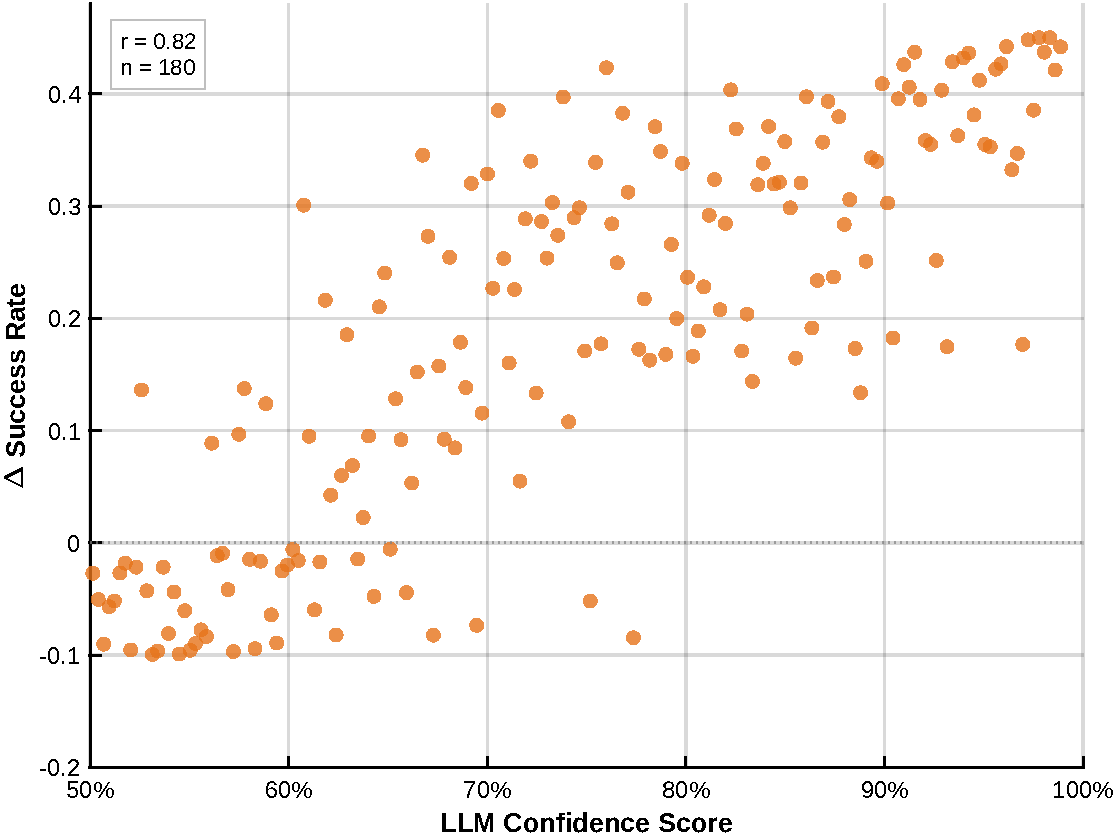
\includegraphics[width=\columnwidth]{figures/confidence.pdf}
\caption{Reported prescription confidence against realised improvement. The confidence
the prescription model reports at prescription time, against the change in the policy's
success rate on the round-level rollout evaluation that the resulting demonstration
produced. GridWorld (image), 180 prescriptions, Pearson $r = 0.82$.}
\label{fig:confidence}
\end{figure}

What makes this number usable, and not a rationalisation after the fact, is the order in
which the two quantities become available. The confidence is reported blind, at
prescription time. At that moment the demonstration has not been collected, the expert
has not been called, the policy has not been retrained, and the re-rollout that produces
$\Delta$SR has not been run. The success-rate signal arrives only after all three of
those steps have completed, by which point the round's unit of budget has already been
spent. The model is therefore forecasting an outcome it cannot observe, and a
correlation of 0.82 to 0.89 is the accuracy of that forecast rather than a description
of an outcome the model was shown.

The number carries two limits, and they are the reason it is reported here rather than
as a result of the paper. The correlation is measured on DISEIL runs only, so it says
nothing about whether a baseline's gate signal would predict its own $\Delta$SR equally
well. And no experiment gates on the confidence: nothing is skipped, deferred or
re-prescribed on the basis of a low score, so the correlation is an observed property of
the system and not yet a mechanism inside it. Turning it into one, by declining to spend
a demonstration on a prescription the model itself does not believe in, has not been
run.

\section{K. Prompts and the Failure Taxonomy}

Every run stores its exact prompts and replies. The material below is a record. The
three model calls are the perception call, the reasoning call and the prescription call.

The perception call takes a system instruction and three frames of a cited failure: the
start of the episode, the flagged step, and the final step.

\begin{figure*}[t]
\centering
\begin{minipage}{\textwidth}
\begin{verbatim}
SYSTEM:  You are analysing a robot manipulation failure from rendered frames. Be
         concrete and spatial; describe what you actually see, not generic advice.

USER:    You are analysing a robot manipulation failure. The attached frames are, in
         order: start, high_loss, end (the peak-loss frame is the policy's
         most-uncertain step, t*=146).
         Task: A UR5e robot with a wiping pad (no fingers) must WIPE a trail
         of dirt markers off the table by pressing down and sweeping along the
         dirt path until all markers are cleared (coverage).
         Describe what went wrong. Focus on: where in the trajectory the failure
         occurs, the robot/gripper configuration at peak loss, and what object or
         contact state caused it. ~120 words, concrete and spatial.
         [start frame] [high_loss frame] [end frame]
\end{verbatim}
\end{minipage}
\caption{The perception call, verbatim from a Wipe run. One defect in the template is
visible and is recorded rather than corrected: the template names the anchor the
``peak-loss frame'', while the frame actually passed is the first-crossing step. The
wording is stale and the frame is correct.}
\label{fig:prompt-vlm}
\end{figure*}

The model's reply on that instance reads: \emph{``The failure occurs during the sweep at
the beginning of the trajectory, around step t*=146. At peak loss, the robot's wiping
pad is positioned at the start of the dirt trail, but the pad is tilted and not fully in
contact with the table surface. The gripper is misaligned, causing the pad to lift
slightly and only partially engage the dirt. This lack of stable contact prevents
effective wiping, leaving the initial segment of the trail untouched.''}

The reasoning call is constrained to the vocabulary of the task's constraint store and
to strict JSON. The closed taxonomy is visible in the prompt: the root cause is one of
six categories and the phase one of five, and the model's job is assignment rather than
invention.

\begin{figure*}[t]
\centering
\begin{minipage}{\textwidth}
\begin{verbatim}
SYSTEM:  You are a robot-manipulation failure analyst. Classify the root cause and
         trajectory phase using ONLY the provided categories and the KAG facts.
         Output strict JSON, no prose, no code fences.

USER:    TASK: {task_description}
         {kag_text}
         VLM FAILURE DESCRIPTION (the only visual evidence): {vlm_report}
         Identify the root cause category and the trajectory phase where the failure
         occurred.
         root_cause in [grasp_failure, approach_failure, placement_error,
                        contact_instability, pose_mismatch, timeout]
         phase      in [pre_grasp, grasp, transport, placement, insertion]
         Output ONLY this JSON:
         {"root_cause": "<one of the categories>",
          "phase": "<one of the phases>",
          "rationale": "<one sentence grounded in the VLM description
                         and a KAG fact>"}
\end{verbatim}
\end{minipage}
\caption{The reasoning call. The two closed vocabularies are read from the task's store
of environmental constraints, so a task that has no insertion phase does not offer one.
The rationale field is what forces the label to be traceable to both the visual evidence
and a named constraint.}
\label{fig:prompt-reason}
\end{figure*}

Its reply on the same failure is the grounding requirement in miniature, because the
rationale cites both the visual evidence and a named node of the store.

\begin{verbatim}
{"root_cause": "contact_instability",
 "phase": "transport",
 "rationale": "The wiping pad tilts
 and lifts during the sweep (transport
 phase) as described in the VLM
 evidence,
 causing intermittent contact with the
 table surface and aligning with the
 KAG-reasoned 'contact_instability'
 failure due to loss of downward
 pressure/alignment."}
\end{verbatim}

The prescription call states the budget rule to the model, offers the two arms of the
prescription, and requires a confidence line.

\begin{figure*}[t]
\centering
\begin{minipage}{\textwidth}
\begin{verbatim}
SYSTEM:  You are a demonstration coach for an interactive imitation-learning
         loop. Each round you spend ONE expert demonstration to fix the
         dominant failure mode. You decide HOW to spend it, grounded in the
         KAG facts and the per-failure analyses.
         Reason briefly, then end with EXACTLY two lines: (1) a decision line
         in the exact required format, and (2) a confidence line
         'CONFIDENCE: <integer 0-100> - <one-line rationale>' reporting how
         confident you are that this demonstration will improve the policy.

USER:    (A) SELECT ep<ID> - one recorded failure represents the whole mode.
             That exact scene is re-run and the expert corrects it on-policy
             from the divergence point t*. Use when the cluster is TIGHT or
             one failure clearly dominates.
         (B) BRIDGE ep<ID>,ep<ID> - no single failure covers the mode.
             Prescribe ONE new object placement in the MIDDLE GROUND between
             2-3 cited failures (e.g. failures at (1,1) and (5,5) -> a demo
             near (3,3)); the expert demonstrates from there.
             Use when the members are geometrically SPREAD but share a root
             cause.
\end{verbatim}
\end{minipage}
\caption{The prescription call. Arm (B) is offered only where the task's constraint
store declares it applicable, so the two arms are read from the store rather than
hard-coded. Wipe declares itself targeted-only and the bridging option is omitted from
its prompt.}
\label{fig:prompt-prescribe}
\end{figure*}

\section{L. Environmental Constraints: Representative Examples}

The store of environmental constraints for a task is a JSON document with a fixed
schema: metadata, typed nodes with key-value properties, relations between them, and a
block of reasoning implications, one per failure mode plus a workspace constraint and a
non-emptiness rule. A renderer turns the document into the text block injected into the
reasoning and prescription prompts. The store is authored once per task, and its
constraints are measurements of the environment rather than opinions about it.

Push-T stores its bounds as typed workspace nodes and its controller as a node in its
own right.

\begin{verbatim}
{"id":"ws_tee","type":"Workspace",
 "label":"Reliable tee init range",
 "properties":{"x":[-0.20,0.20],
               "y":[-0.25,0.05],
               "z":0.021}},
{"id":"ws_tcp","type":"Workspace",
 "label":"Reliable tcp range",
 "properties":{"x":[-0.35,0.35],
               "y":[-0.35,0.35],
               "z":[0.02,0.08]}},
{"id":"ctrl","type":"Controller",
 "label":"pd_joint_pos /
           rel_joint_pos",
 "properties":{
   "policy_action":"7 joint deltas
                    (rel_joint_pos)",
   "expert_action":"PPO ->
        joint_delta_pos (same
        7-joint space)"}}
\end{verbatim}

The predicate the feasibility loop checks is stored as an implication and is written in
the imperative, because it is addressed to the model as much as to the checker.

\begin{quote}
\raggedright
\texttt{"workspace\_constraint": "Every prescribed config MUST keep tee\_xyz within
x[-0.20,0.20] y[-0.25,0.05] z=0.021 and tcp\_xyz within x[-0.35,0.35] y[-0.35,0.35]
z[0.02,0.08]; out-of-range poses are dropped (the PPO expert is unreliable there) and
waste the round."}
\end{quote}

That constraint is also where the Push-T expert's partial competence is encoded. The
expert pushes in one rotational direction only, so the configurations it cannot
demonstrate are excluded before a prescription is issued rather than discovered after
the expert has failed on one.

Door's constraint is tighter by an order of magnitude, and the numbers are a padded
empirical measurement of the simulator's own reset sampler, so that a prescribed
configuration cannot leave the task's native reset distribution.

\begin{verbatim}
{"id": "ws_door", "type": "Workspace",
 "label": "Reliable door-frame range",
 "properties": {"x": [-0.135, -0.108],
                "y": [-0.366, -0.340],
                "z": 1.10,
                "yaw_rad":
                    [-1.82, -1.57]}},
{"id": "succ",
 "type": "SuccessCondition",
 "label": "Door open",
 "properties": {
   "metric": "hinge_qpos > 0.3 rad",
   "info_key": "success"}}
\end{verbatim}

For a discrete task the environmental constraint is not a bounding box but a
reachability predicate, and GridWorld's store states it as one. A prescribed layout must
place the start cell, the goal cell and the three obstacle cells as distinct in-grid
cells, with a minimum separation between start and goal and a breadth-first path from
one to the other that avoids the obstacles. A layout that fails the predicate is
rejected before it reaches the expert.

Wipe shows the store doing something a bounding box cannot do at all. Its document
carries an implication that removes an entire arm of the prescription from the task.

\begin{quote}
\raggedright
\texttt{"select\_only": "Wipe randomizes a whole marker PATH, not a single object pose,
so BRIDGE is infeasible - always choose SELECT of the most representative failed
episode."}
\end{quote}

The planner reads that implication structurally and the prompt omits the bridging
option. The store therefore does two jobs. It constrains where a demonstration may be
placed, and it determines which prescription arms exist for a task at all. Both jobs are
done by knowledge that is written down and checkable, which is the sense in which the
framework's model of the environment is explicit rather than implicit in a network's
weights.

\section{M. Qualitative Examples and Failure Cases}

\paragraph{The modes the partition discovers.} Figure~\ref{fig:modes} shows the three
failure modes discovered on Push-T (image) with three sampled members of each. The modes
are behaviourally distinct: the block is brought to the goal region but left almost fully
inverted; the arm never establishes a working contact; the block is pushed but abandoned
at a moderate orientation error and far from the end-effector. The clusters are found
from geometry alone and the naming pipeline supplies their labels from the task store's
own vocabulary. Three is not the number of failure modes on these tasks. It is the count
most often selected when the silhouette criterion runs, and the count varies by round, as
study A15 reports.

\begin{figure*}[t]
\centering
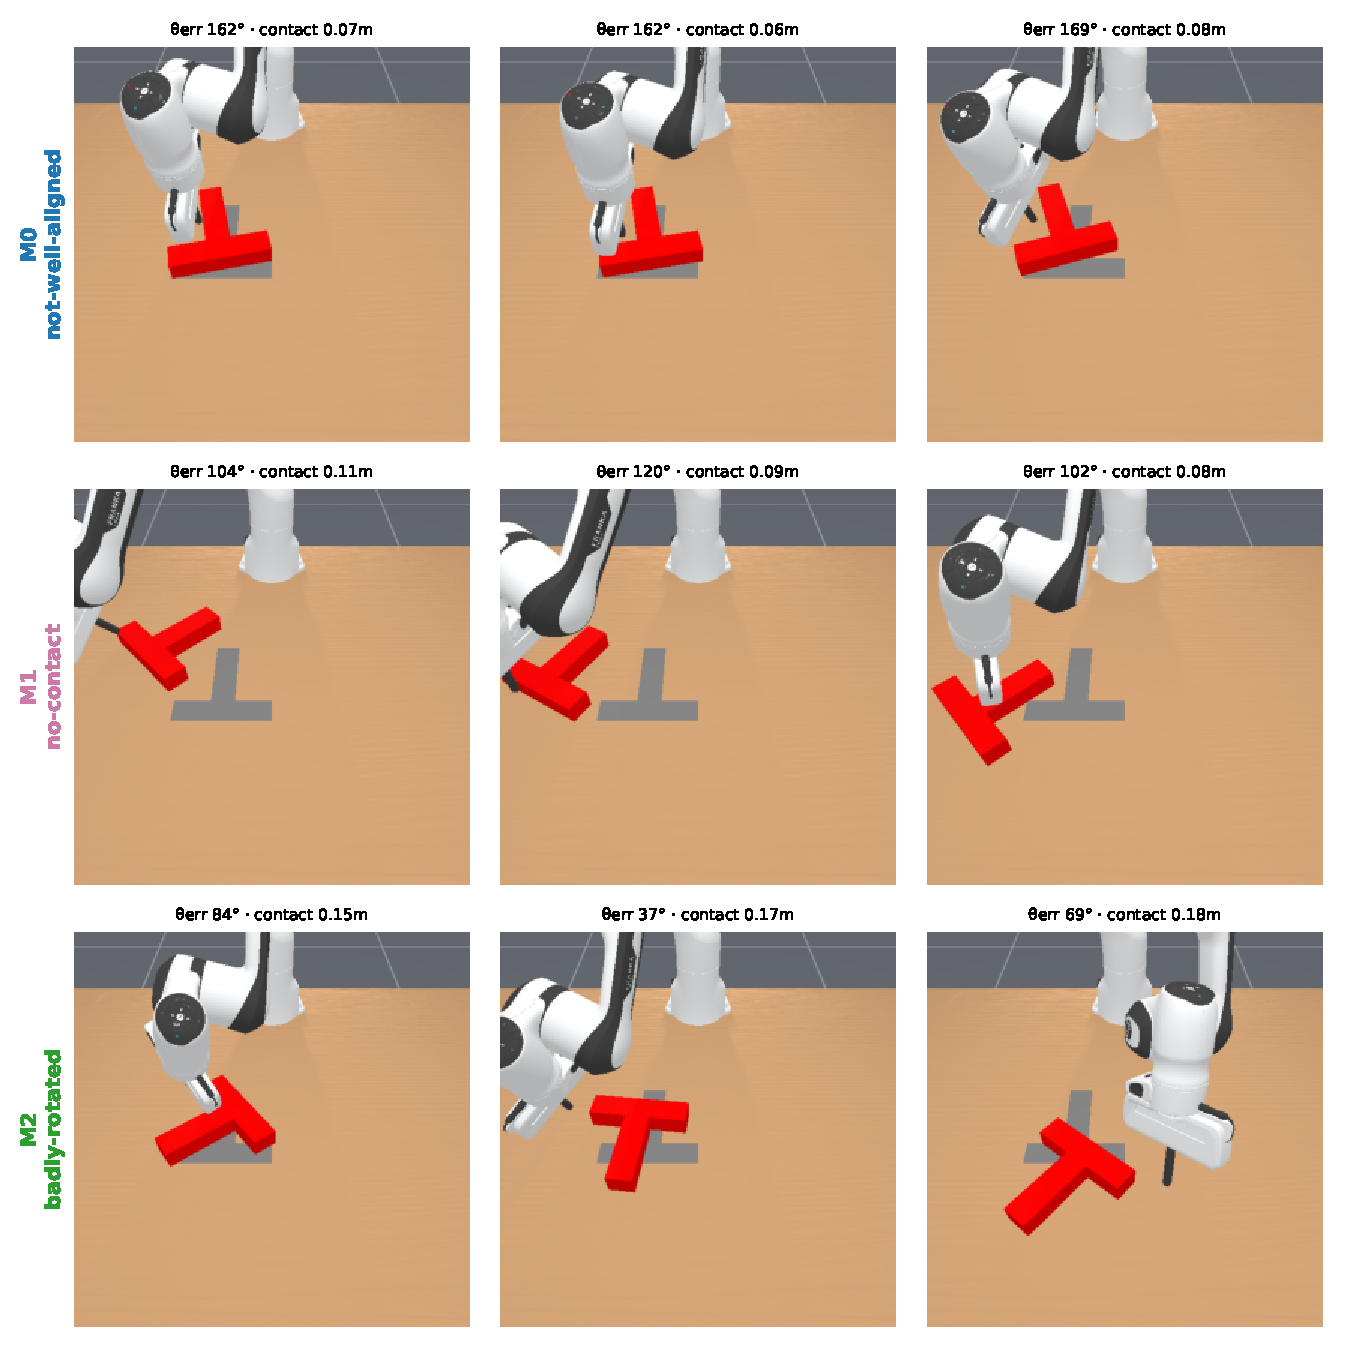
\includegraphics[width=\textwidth]{figures/failure_modes.pdf}
\caption{Failure modes discovered on Push-T (image). Each row is one geometric cluster of
the round's recorded failures, with three sampled members. Labels are assigned by the
naming pipeline from the task store's vocabulary. The figure illustrates the object the
framework allocates over; the evidence that the partition buys the result is study A3.}
\label{fig:modes}
\end{figure*}

\paragraph{A round, end to end.} The cited failures are handed to the prescription model
one line each and the model answers in two lines. The round below is taken verbatim from
a Wipe log.

\begin{verbatim}
DOMINANT FAILURE CLUSTER
(members with their VLM+analysis
findings):
  - ep3000001:
      object_xy=(0.221,-0.027)
      progress=74/500
      peak_loss=0.0434
      root_cause=contact_instability
      phase=transport
  - ep3000003:
      object_xy=(0.165,-0.068)
      progress=146/500
      peak_loss=0.0181
      root_cause=contact_instability
      phase=transport
  - ep3000006:
      object_xy=(0.123,-0.157)
      progress=234/500
      peak_loss=0.0186
      root_cause=pose_mismatch
      phase=placement
===== RESPONSE =====
SELECT ep3000001
CONFIDENCE: 85 - Ep3000001's
contact_instability root cause (higher
peak_loss) at early progress best
represents the dominant failure mode,
ensuring the expert demonstration
directly addresses unstable wiping
pressure causing missed coverage.
\end{verbatim}

\paragraph{An impure cluster, from the inside.} That record also shows the imperfection
of a geometric partition. Two of the three cited members carry the label
\texttt{contact\_instability} and the third carries \texttt{pose\_mismatch}, so this mode
has a purity of two thirds. The purity measured across the ablation settings, 0.84 to
0.91 in study A14, is an average over instances like this one, and the failure case is
the one A14 describes in aggregate: the third episode is at a similar place in the
workspace and arrived there by a different process, and geometry cannot separate the two.
The prescription in this round is unaffected, because the selected episode is a member of
the majority cause, but nothing in the framework guarantees that.

\paragraph{The failure cases the framework has.} Four are visible in the record above and
in the studies. A cluster can carry more than one root cause, which A14 measures and the
example illustrates. A round can fail to produce a feasible prescription within
$J_{\max}$ attempts and fall back on the nearest untried failure, which happens in 27 to
35 per cent of rounds once the constraint store is removed and which A6 prices. A round
can have too few failures to partition at all, which happens in 15 to 21 per cent of
rounds and concentrates at the end of the budget, which A15 and A17 measure. And a task
can begin the budget above the band in which allocation matters, which is what Lift does
and why Lift is uninformative about any mechanism.

\section{N. Extended Limitations and Outstanding Items}

The main paper states the limitations that bound its claim. This section states them in
full, ordered by how much they constrain the claim, and then lists the items that are
open.

\paragraph{The selector reasons about one round and knows nothing about the dataset.}
The selector consumes the current policy's failures, partitions them into failure modes,
and prescribes one demonstration. Its only representation of history is the
recency-discounted penalty applied to the clusters already corrected, which records
\emph{where} corrections have been placed in the descriptor space and holds no
representation of \emph{what the training set contains}. The consequence bounds the
framework's central objective. The selector can determine that the policy failed at a
particular configuration and that the root cause is, say, a grasp failure. It cannot
determine that the training set already holds six demonstrations of that cause, and that
the failure is therefore a symptom of under-fitting and not of under-coverage. Under a
restricted budget, a demonstration spent re-teaching material the dataset already
contains is a demonstration lost, which is the opposite of what the budget exists to buy.
Nothing in the current instantiation prevents that expenditure and nothing in it measures
how often it occurs. The gap is not closed by the cluster memory even in principle: a
memory indexed on geometry answers ``have we placed a demonstration near here?'' and not
``does the dataset already contain this behaviour?'', and the two questions come apart
wherever geometry does not determine cause, which A14 measures directly. Retrieval methods index a corpus
by embedding distance and select from it \citep{memmel2025strap}; others reweight a
corpus by domain \citep{hejna2024remix} or score it by quality
\citep{belkhale2023dataquality}. This framework has no such index, and its selector was
never given one.

\paragraph{The descriptor is designed by hand, and geometry recovers cause only where
configuration determines cause.} A10 defends the descriptor's \emph{width} on a criterion
independent of the reported success rates, and what it establishes is that within this
family of geometric features six dimensions is the right number. It says nothing about
whether a learned descriptor, of the kind that frozen visual encoders supply for the
image-modality policies \citep{nair2022r3m}, would separate failure modes better. That
experiment has not been run. A14 locates the descriptor's ceiling, and purity is measured
against the prescription model's own labels and covaries with silhouette, so neither
measurement audits the other. A human-labelled root-cause set is the measurement that is
missing.

\paragraph{The cluster memory is worth about three quarters of a point, and how much
depends on the task.} No study establishes when a task should switch it on. The three
settings disagree by a factor of three, three settings cannot support a rule, and the
rule is not offered.

\paragraph{Each language-model component is worth about one and a third points, for a
structural reason.} The comparison that sharpens the point is the grounding knockout:
removing the prescription model costs 1.33 points, and removing the environmental
constraints against which its proposals are verified costs 2.37 and drives the fallback
rate to between 27 and 35 per cent of rounds. Two readings are admissible, that language
models add little to demonstration selection, or that the language model here was given
too little to reason over. The evidence supports the second. The literature says why this
should be expected, since vision-language models are reliable at naming a cause given
structured evidence and unreliable at metric geometry from pixels alone
\citep{chen2024spatialvlm, fu2024blink}. The framework hands the model a low-dimensional
geometric descriptor and a constraint store for exactly that reason, and it then does not
hand it anything else.

\paragraph{The allocation machinery is active early and idle late.} Failures per round
fall from forty-two to two, and below four remaining failures the sweep is skipped.
Across the three ablation settings, 15 to 21 per cent of all rounds skip clustering. The
allocation account is an account of the early and middle rounds, and the failure-count
curve is instrumented on one setting only.

\paragraph{The reasoning pipeline costs seconds and tokens.} The add-on the baseline
never pays is 63 seconds per round at the cheapest setting and 1,232 at the most
expensive, at 9,560 to 82,116 tokens. The round ratio of 1.13 to 2.75 is the smaller of
the two facts, because the retrain and the evaluation that both arms pay dilute it. A
ratio near one measures the retrain's expense, not the pipeline's cheapness.

\paragraph{The experiments are in simulation and no expert is a person.} Every result
comes from simulation with an expert that answers instantly and correctly, and charges
the same for any prescription. The uniformity assumption is what allows the
budget to be counted in demonstrations. Outside simulation the budget is a person's time,
demonstrations differ by an order of magnitude in what they cost to produce, and human
demonstrators are not uniformly correct
\citep{belkhale2023dataquality, khazatsky2024droid, mandlekar2020iwr,
mandlekar2018roboturk}. The second half of the information-gain argument fails the moment
the demonstrator is a person, because high pre-retrain loss identifies novel data only if
invalid demonstrations are ruled out by construction.

\paragraph{Outstanding items.} Five are open and none is resolved by an assumption. The
bridging discrepancy of A16, in which 24 per cent of GridWorld prescriptions are marked
bridged on a discrete grid, awaits an inspection of the prescription logs. The
decomposition of the constraint store, which A6 does not perform, leaves it unknown
whether the workspace bounds alone would recover most of the damage. The cleaner variant
of A3, which keeps the descriptor and replaces agglomerative clustering with a random
partition into $k$ groups, was not run, so A3 knocks out the allocation stack rather than
the partition in isolation. The solvability screen is not exercised in any reported run
and is not ablated anywhere. And the failure-count instrumentation of A17 exists on one
setting, so the front-loading behaviour is not claimed as general.

\bibliography{references}

\end{document}
